% Document class options:
% =======================
%
% lineno: Adds line numbers.
%
% serif: Sets the body font to be serif. 
%
% twocolumn: Sets the body text in two-column layout. 
% 
%
% Using other bibliography styles:
% =======================
% Not supported at the moment
\documentclass[twocolumn, serif, rga, numeric]{jote-article}

\usepackage{sourcesanspro}
%%% Add the bibliography, make sure it's in the same directory
\addbibresource{bekkers.bib}

%%% Add additional packages here if required. Usually not needed, except when doing things with figures and tables, god help you then

% This package is for generating Lorem Ipsum, usage: \lipsum[X] where X is the Xth paragraph of lorem ipsum. OR use [1-5] to generate the first five, etc.
\usepackage{lipsum}


% Fill in the type of article here. Doesn't matter if capitalized. 
%%% Options
% Empirical
% Reflection
% Meta-Research
% Rejected Grant Application
% Editorial

%%% TODO: Make this a 1-5 option scale to reduce the chance of mistyping
\papertype{Rejected Grant Application}

% Enter the title, in Title Case Please
% Try to keep it under 3 lines
\title{Global Giving}

% List abbreviations here, if any. Please note that it is preferred that abbreviations be defined at the first instance they appear in the text, rather than creating an abbreviations list.
%\abbrevs{ABC, a black cat; DEF, doesn't ever fret; GHI, goes home immediately.}

% Include full author names and degrees, when required by the journal.
% Use the \authfn to add symbols for additional footnotes and present addresses, if any. Usually start with 1 for notes about author contributions; then continuing with 2 etc if any author has a different present address.
\author[1]{Ren\'e H. F. P. Bekkers }
%Fill it in again for the PDF metadata. Lame workaround but it works
\authorone{Ren\'e Bekkers}

\usepackage{enumitem}% http://ctan.org/pkg/enumitem
\setlist[itemize]{noitemsep, topsep=0pt, labelindent=\parindent, leftmargin=2\parindent, label=$\triangleright$}
\setlist[description]{noitemsep, topsep=0pt}
\usepackage{pifont}

%List the contribution effort here, they will be listed at the end of the page
%List the acknowledgments. If there is no companion piece, this is listed below the author info
%List possible conflict of interest. Will default to saying no conflict exists.

% Include full affiliation details for all authors
\affil[1]{Center for Philanthropic Studies, Department of Sociology, Faculty of Social Science, Vrije Universiteit Amsterdam}
%\affil[2]{The streets}

% List the correspondence email of the main correspondent
\corraddress{Ren\'e H. F. P. Bekkers, Center for Philanthropic Studies, Department of Sociology, Faculty of Social Science, Vrije Universiteit Amsterdam, De Boelelaan 1105, Amsterdam, 1081 HV, The Netherlands}
\corremail{\href{mailto:r.bekkers@vu.nl}{r.bekkers@vu.nl}}
\rgainfo{Netherlands Organisation for Scientific Research Vici scheme 2019}

% Optionally list the present address of one of the authors
%\presentadd[\authfn{2}]{Department, Institution, City, State or Province, Postal Code, Country}

% Fill in the DOI of the paper

% Always starts with "10.36850/" and is suffixed with one of the following plus a number
% e  : empirical
% r  : reflection
% mr : meta-research
% rga: rejected grant application
% ed : editorial
\paperdoi{10.36850/rga2}

% Include the name of the author that should appear in the running header
\runningauthor{Bekkers}

% The name of the Journal
\jname{Journal of Trial and Error}

% The year that the article is published
\jyear{2020}

%The Volume Number
\jvolume{1}
\jissue{1}
\jpages{72-100}

%The website that's listed in the bottom right
\jwebsite{https://www.jtrialerror.com}

%%% Only \paperpublished is necessary, any combination of the other two is possible

%When the paper was received
\paperreceived{19 May, 2020}
% When the paper was accepted
%\paperaccepted{2 January, 2020}
% When the paper will be published
\paperpublished{2 December, 2020}
% When the paper is published but in YYYY-MM-DD format, for the crossmark button
\paperpublisheddate{2020-12-2}

% The pages of the article, comment out if rolling article
%\jpages{1, -12}
% Link to the logo, might be redundant
\jlogo{media/jote_logo_full.png}

% Fill something here if this is a rolling/online first article, will make ROLLING ARTICLE show up on the first page
%\rolling{YES}

% Sets the paragraph skip to be zero, this should be in the CLS
\setlength{\parskip}{0pt}
\usepackage[table]{xcolor}
%%% Companion Piece

% Reflection and Empirical articles have each other as companion pieces. Add the DOI, Title, and Abstract of the respective Companion piece here
%\companionurl{https://doi.org/10.36850/rX}
%\companiontitle{Author Three (2020)\newline Very Serious Reflection}
%\companionabstract{\noindent \lipsum[6]}

%%% Abstract

% These two set the height and width of the abstract. There's no solution to do this automatically at the moment so fiddle with these a bit. height-width should be 5mm, and ranges between 50-100 are realistic
% Higher number means skinnier abstract
\heightabstract{40mm}
\widthaffil{35mm}
%Enter something here in order for the abstract to disappear. Be sure to also delete the abstract 
\noabstract{}
% Fill in the keywords that will appear in the abstract, max 7
\keywordsabstract{philanthropy, charitable giving, cooperation, international comparative research}


%%%%%%%%%%%%%%%%%%%%%%%%%%%%%%%%%%%%%%%%%%%%%%%%%%%
%Document Starts
%%%%%%%%%%%%%%%%%%%%%%%%%%%%%%%%%%%%%%%%%%%%%%%%%%%
\reversemarginpar
\begin{document}
\setcounter{page}{72}
\pdfbookmark[0]{Bekkers, R. - Global Giving}{nelsonpdf}

%%% This starts the frontmatter, which includes everything that's on the front page execpt the text of the article
\begin{frontmatter}
\maketitle
%Type your abstract between these things. Max 250 words. Be sure to include the \noindent, looks bad otherwise
\begin{abstract}
Why do citizens in some countries take more responsibility for the well-being of others than in other countries? This project seeks to understand the genesis of prosociality, investigating its biological foundations, the influence of cultural traditions, and effects of political, economic and legal structure. The dominant theory in economics views philanthropy as a solution to social illnesses that the market and the state are not solving, a view complementary to political science theory on preferences for government provision. Sociologists focus on social norms emerging from religious traditions. Cultural evolutionary theory highlights the instrumental value of trust. Still other theories have suggested a role for natural selection of genes.

However, these theories have not been tested stringently nor simultaneously. Also the project includes a very important factor largely ignored thus far: political, legal and economic institutions also affect the level of giving as well as who gives to which causes.
Therefore, the objectives of Global Giving are (1) to map country differences in the size and nature of philanthropy across the world; (2) to develop and test multidisciplinary theories explaining these differences; (3) to facilitate international collaboration across disciplinary boundaries in research on philanthropy. The research draws upon 200 surveys recently harmonized by the PI and on new data on philanthropy to be collected among large samples in 145 countries across all continents. Collaboration with international networks of academics safeguards the validity of the questionnaires and experiments. Appropriate multilevel regression models will be used, the lack of which caused biases in previous research.

An integrated understanding of philanthropy is useful not only for theory development, but also for government policy makers and practitioners in nonprofit organizations seeking to mobilize philanthropic contributions and make them more effective. The application in practice is ensured through collaboration with a large network of practitioners.
\end{abstract}
\end{frontmatter}





%\begin{longtable}[]{@{}ll@{}}
%\toprule \begin{minipage}[b]{0.47\columnwidth}\raggedright \hfill\break \strut \end{minipage} & \begin{minipage}[b]{0.47\columnwidth}\raggedright \hfill\break \strut \end{minipage}\tabularnewline \midrule \endhead \begin{minipage}[t]{0.47\columnwidth}\raggedright \hfill\break \strut \end{minipage} & \begin{minipage}[t]{0.47\columnwidth}\raggedright \begin{quote}
%Netherlands Organisation 
%for Scientific Research \end{quote}\strut \end{minipage}\tabularnewline \bottomrule \end{longtable}
%Netherlands Organisation for Scientific Research
%Vici scheme application 2019

\phantomsection \addcontentsline{toc}{section}{Research proposal}\section*{Research proposal} 
\vspace{\baselineskip}
\phantomsection \addcontentsline{toc}{subsection}{General information}\subsection*{General information}

\subsubsection*{Institution of employment at time of application}

Center for Philanthropic Studies, Department of Sociology, Faculty of Social Sciences, Vrije Universiteit Amsterdam

\subsubsection*{Prospective host institution}

Center for Philanthropic Studies, Department of Sociology, Faculty of Social Sciences, Vrije Universiteit Amsterdam

\subsubsection*{Main field}

Sociology 
\phantomsection \addcontentsline{toc}{subsubsection}{Other fields}\subsubsection*{Other fields} 

Social and Organizational Psychology, Political Science, Macroeconomics, Public Administration 
\phantomsection \addcontentsline{toc}{subsubsection}{Explanation of the multidisciplinary character of the proposal}\subsubsection*{Explanation of the multidisciplinary character of the proposal} 

Societies do not neatly observe the boundaries between academic disciplines, and neither do people. Giving can be a political act; it can be religiously motivated; it can be a form of conspicuous consumption; and it may spring from humanitarian concerns. The same gift can result from all of these. Yet different disciplines have focused on explanations at different levels, and with particular clusters of determinants. Political science has understood philanthropy as political behavior based on liberty and democratic institutions. Sociology has emphasized cultural traditions, trends and social influences at the national and social group level; social and organizational psychology has studied group processes and the behavior of individual citizens.
Biologists have explained philanthropy as an extreme form of altruism resulting from evolutionary processes selecting for certain genetic polymorphisms. In reality, these factors are all interwoven in a complex web of determinants. To explain cross-national differences in philanthropy, monodisciplinary explanations are incomplete. We need to understand how individual motivations and societal circumstances interact. For instance, personality and self-identity theories explain giving as the result of individual traits with genetic underpinnings, while institutional theories suggest that such traits matter only for individuals in groups that are actively mobilized.

\subsubsection*{Number of words}

Description of the proposed research: 7,957 (max. 8,000 words)

\noindent Knowledge utilisation: 849 (max. 1000 words)

\phantomsection \addcontentsline{toc}{subsection}{Description of the proposed research}\subsection*{Description of the proposed research} 

This proposal and background materials are publicly available at \url{https://renebekkers.wordpress.com/global-giving/}

Why do citizens in some nations give more money, time and other resources to the benefit of society than citizens in other nations? How can these differences between nations be explained? \emph{Global Giving}
moves the frontier of research beyond the focus on western countries and narrow mono-disciplinary accounts that dominate the literature today.
Going beyond micro-level theories that explain who gives what and why, \emph{Global Giving} will provide an integrative multidisciplinary explanation of cross-national differences in generosity, adding institutionalization and organization of the non-profit sector as macro-level context factors. Also the research will improve the methods and statistics currently used in behavioral social science research.

To do so, \emph{Global Giving} will (1) map country differences in the size and nature of philanthropy among large (\emph{n} \textgreater{}
1,000) representative samples across a large number (145) of countries; (2) develop, operationalize, and test theories explaining differences in philanthropy between countries; (3) facilitate international collaboration across disciplinary boundaries in research on philanthropy and provide methodological innovations that will benefit researchers in the social sciences as a whole.

Philanthropy -- the voluntary contribution of private resources to collective welfare \cite{Smith2006} -- is an increasingly important social behavior contributing to the well-being of citizens in nations across the world. Governments are calling upon citizens and corporations to take responsibility for society as a whole. Engagement in philanthropy has been linked to better health and well-being of the giver \cite{Aknin2013, DeWit2015, Dunn2008, Konrath2012} but more importantly, society benefits from generosity. Recent history provides dramatic examples of the contribution of philanthropy to a better world. Long before the international community came to a coordinated response, nonprofit organizations such as Unicef and Doctors Without Borders provided emergency shelter, food, and health care to victims of the civil war in Syria. The first Ebola vaccine was produced in a lab funded by the Wellcome Trust. Through coordinated efforts supported by a coalition of the WHO, Unicef, and the Rotary International Foundation, polio was eradicated from Africa. The Ocean Cleanup system was recently launched to remove plastic waste from the oceans. In countries like Greece, still suffering from the economic downturn, volunteers in churches and welfare organizations provide for basic needs through soup kitchens and food banks.

Across the globe, countries differ markedly in the prevalence of philanthropy, as Figure \ref{fig:map} shows. Such behavioral differences in prosociality are at the heart of \emph{Global Giving}. Countries with high levels of engagement in philanthropy are the Netherlands, Ireland and the UK (75-80\% giving to charity), Australia and New Zealand (around 70\%), and the US and Canada (60-65\%). Much lower levels of engagement in philanthropy are found in Russia and China (5-10\%), India and Japan (\textasciitilde25\%). Also within Europe we find considerable differences, where citizens in the Netherlands, the UK and Ireland, are 8 times more likely to engage in philanthropy than citizens in Lithuania, Russia or Greece. Where do these differences come from? How can they be explained? Are the differences indicative of generosity, or do they merely reflect economic prosperity? Due to a lack of data these questions cannot be answered. The data in Figure \ref{fig:map} say nothing about the amounts donated. In the Netherlands, the only country beyond the US where such a figure is available, philanthropy amounts to about 0.8\% of GDP \cite{Bekkers2015b}. So while the Netherlands may seem to be a generous country in Figure \ref{fig:map}, the amounts donated in acts of giving tend to be small for most households \cite{Bekkers2015b}. In the US, philanthropy amounts to about 2\% of GDP \cite{Foundation2014}.

\begin{figure*}[t]
    \centering
    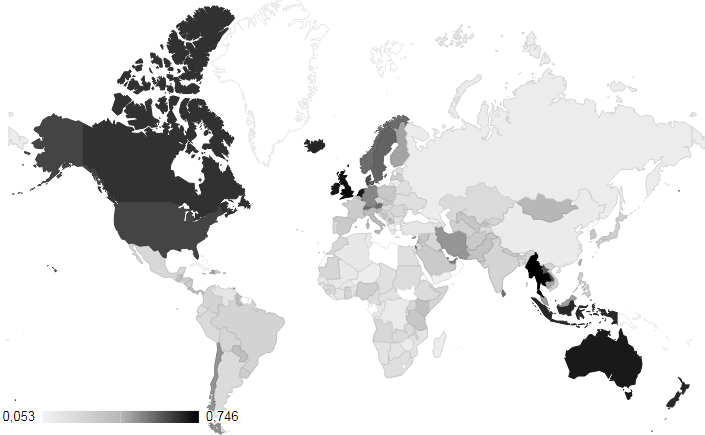
\includegraphics[width=\textwidth]{articles/RGAs/bekkers/map.png}
    \caption{Country differences in the incidence of charitable giving (\% of population donating to charity, 2010-2017 average).
Source: CAF \cite{CharitableGivingFoundation2010}\emph{own computation}}
    \label{fig:map}
\end{figure*}

An attempt to harmonize existing data on philanthropy from various countries in the world in the International Philanthropy Database (IPD) \cite{Wiepking2015} concluded that a comparative analysis of amounts donated is difficult. As a result, previous comparative research on philanthropy is limited to analyses of the likelihood that citizens donate money to charity \cite{Bekkers2016}.

Theoretical models of philanthropy discussed below have focused at the individual level and have been developed in western countries. They suggest that different motivations underlie the decision to give money and the amount donated. However, it is unclear how prevalent these motivations are in different countries. This is important to know because academic research on philanthropy has been conducted primarily in western countries. While philanthropy is an increasingly global phenomenon, the use of `WEIRD' samples of WEstern, Industrialized, Rich and Democratic participants limits the generalizability of existing research \cite{Henrich2010}. The generalizability of research on philanthropy is also limited because of the overwhelming influence of seemingly trivial context factors \cite{Guala2010, Tammi2013}.
Experiments with charitable giving as an outcome variable have produced widely different results as a function of minimal differences in the design of these experiments.

Motivations for giving are likely to differ between countries. But before we can even begin to answer the question how characteristics of countries affect motivations for giving, it is important to know the basic numbers: where do which citizens give what to which causes? 
The global increase in charitable giving in the wake of the economic recovery after the financial crisis suggests that improvements in the economy can increase giving across societies \cite{Bekkers2015b}.
However, even long periods of economic growth and strong increases of wealth have not increased philanthropy in China, India and Russia by much, and the ranking of countries has remained about the same. Why are people living in countries such as the Netherlands, the UK, the USA, Canada, Australia and New Zealand much more likely to give to charity? What proportion of income and wealth are donated in these countries? Are relative levels of generosity there also higher than in other countries? 
\phantomsection \addcontentsline{toc}{paragraph}{Overview}\paragraph{Overview.} 

The research I propose on country differences in philanthropy is based on an integrated model of giving behavior involving determinants at three levels, displayed in Figure \ref{fig:lobster} \cite{Penner2005}. The model departs from macro-level differences between countries in values and institutions in the top left corner, which affect meso-level differences in the activities of nonprofit organizations about mobilization strategies (arrow A). The strategies of nonprofit organizations, in turn, are attuned to and affect the likelihood that individual citizens will be asked to contribute, and the characteristics of the situations in which they are asked (arrow B). For individual citizens, the decision to give is influenced by the characteristics of the giving situation and their resources and prosocial values (arrow C). Both the organizations that solicit contributions (arrow B) as well as the national context in which individual giving decisions are made (arrow D) affect the nature and level of giving. They also affect the influence of situational and individual donor characteristics (arrows E and F).
\begin{figure}
    \centering
    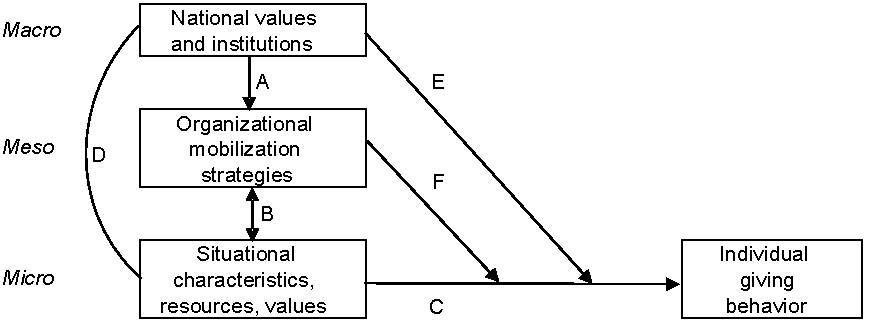
\includegraphics[width=\columnwidth]{articles/RGAs/bekkers/lobster.pdf}
    \caption{Three level model of giving behavior.}
    \label{fig:lobster}
\end{figure}


The simultaneous consideration of factors at three levels is a novel contribution to the field of research on philanthropy. While the three-level model is commonly used in research on education, stratification and health, most of the academic research on giving behavior has been limited to characteristics at the micro-level \cite{Bekkers2007, Bekkers2016a}. For social scientists, however, the enormous differences between countries in the proportion of the population engaging in philanthropy that the map in Figure \ref{fig:map} shows pose intriguing questions. Why do some countries have much lower proportions engaging in philanthropy than others? How much do people give as a proportion of their income and wealth in countries around the world? How can country differences in generosity be explained? Could situational characteristics that increase generosity in western countries be leveraged in non-western countries? The research I propose is the first to answer these questions. It is also relevant for practitioners in nonprofit organizations. Knowledge on situational characteristics and organizational strategies that make people give are obviously of interest to organizations that collect contributions.
\emph{Global Giving} will show how factors that drive giving differ between countries.

\phantomsection \addcontentsline{toc}{subsubsection}{Theory}\paragraph{Theory.} 

Philanthropy is a unique form of human cooperation. It poses a puzzle: in contrast to informal helping, it cannot be explained from principles of reciprocity \cite{Rand2015}. People help their neighbors, friends and family, both in their current country of residence and in their country of origin through remittances. People even help strangers by doing things for them, or indirectly by giving them access to their resources. These are examples of \emph{informal giving} because there is no formal organization involved. Informal giving can be explained by kinship altruism, \cite{Dawkins1976, Hamilton1964} direct reciprocity and exchange \cite{Blau1964, Homans1958}. However, people also engage in cooperation by giving time to nonprofit organizations by volunteering, donating money to charitable organizations and giving blood to blood banks. These examples of giving all involve an intermediary organization that channels the help offered by individuals to the beneficiaries. Even though friends and family often raise funds for charitable causes in their direct social environment, acts of philanthropy cannot be driven entirely by direct reciprocity, and require different explanations \cite{Moody2008, Gouldner1960, Gouldner1973}.

\emph{Global Giving} focuses on such acts of formal giving. In these acts people usually do not have direct contact with the beneficiaries, and they cannot be sure that their efforts will be compensated in the future. In these cases, philanthropy does not hold the promise to the donor that once she will be the beneficiary of an act of reciprocated giving. Because direct reciprocity is unlikely to explain formal giving it poses an intriguing puzzle for social science.

That said, there is no dearth of theories explaining philanthropic behavior, especially at the micro-level. Philanthropy is so multi-faceted that it cannot be explained by a single theory, but requires a multidisciplinary perspective \cite{Brown1997, Dovidio2006}.
Therefore, an important aim of the current research is to synthesize the theories that purport to explain philanthropy in different disciplines.
In addition, we draw special attention to theories that identify factors at the meso- and macro-levels of analysis, because they have been ignored in previous research and hold the key to explain cross-national differences.

\paragraph{Micro-level theories: Who Gives When?}

Researchers have tried to solve the puzzle of philanthropy in two different ways, each with its own type of explanation and methodology.
The first type of explanation uses as evidence answers to the question `who gives?' In this strand of research, random sample surveys are often used to measure the tendency of a large number of people to engage in philanthropy through a series of questions on various forms of giving, including donations to charity and volunteering. The second type draws upon answers to the question `when do people give?' In this strand of research, specific examples of giving are observed among small samples of participants in experiments that manipulate situational characteristics. An important contribution of \emph{Global Giving} is that these two types of explanations will be combined, and investigated in conjunction with explanations for country differences.

\subparagraph{1. Who gives?}

\ \ Broadly speaking, two groups of factors dominate the literature on characteristics of charitable donors and countries: resources and values. At the individual level, citizens with more resources at their disposal in the form of human and social capital and with stronger prosocial values give more.

\emph{Resources.} As charitable giving is costly, those with more resources at their disposal will be more likely to engage in it \cite{Wilson1997}. There is a broad consensus in research relying on surveys that education, status and income are positively correlated to charitable giving \cite{Bekkers2011d, Korndorfer2015, Wiepking2012}. The level of education is one of the ubiquitous correlates of charitable giving.
In all countries where this relation has been investigated, higher educated citizens are more likely to contribute and give more \cite{Bekkers2011d}. Analyses of donations using data from income tax returns and longitudinal panel surveys in the Netherlands and the USA show that as their income and wealth increase citizens spend higher amounts on giving, but a lower proportion of income \cite{Bekkers2009, Duffy2015}. Results from several other countries tend to be similar \cite{Wiepking2012}. In my previous research I have used life course data and genetically informed designs to examine how the relationship between the level of education and philanthropy can be explained within countries \cite{Bekkers2014, Bekkers2008a}. To some extent, the correlation between the level of education and the amount donated is due to higher levels of income and wealth accumulated \cite{Wiepking2009} but controlling for them does not diminish the relationship to zero \cite{Bekkers2011d}. Charitable giving is also dependent on resources of others accessed through social networks \cite{Wiepking2009, Glanville2016}. To some extent, social capital explains why human capital is associated with charitable giving \cite{Wiepking2009}. Also the relation between religious affiliation and philanthropy is reduced when social capital is taken into account \cite{Bekkers2008}.

\emph{Prosocial values.} While resources increase the budgets that constrain the giving behavior of individual citizens, they do not give a positive explanation of why they give, and how generously they give relative to their budgets. Charitable giving will only occur when people prioritize helping others and collective welfare. The moral principle of care, the internalized value that citizens attach to helping others \cite{Batson1994, Hoffman2000} is thus an important correlate of charitable giving and a variety of prosocial behaviors in daily life \cite{Wilhelm2010}. The principle of care may also be able to explain why some people are more generous than others and why members of religious groups give more. As all major religions stress the moral value of helping others, it is likely that the principle of care explains a part of the remaining relationship between religious affiliation and charitable giving. The \emph{Global Giving Survey} will be the first survey to study the giving behavior of members of non-western religious groups in conjunction with the moral principle of care. In addition, generalized social trust is an important trait of citizens who engage in prosocial behavior \cite{Bekkers2003, Uslaner2010}.

\subparagraph{2. When do people give and why?}

\ \ Research on philanthropy commonly contrasts purely altruistic motivations to give with `impure' or `egoistic' motives, sometimes labeled `warm glow'\cite{Andreoni1990}. The hypothesis of pure altruism states that the desire to help others, if aware and given the opportunity to have an impact, leads individuals to adapt their level of giving to the societal need for contributions. Experiments finding that most participants do not do so proportionally is taken as evidence for non-altruistic motivations for giving, as if people derive utility from the act of giving and not so much from the increase in well-being among recipients of donations \cite{Ribar2002, deWit2016, Vesterlund2006}. The reasons why people enjoy the act of giving more so than the increase in the well-being of recipients include social image concerns (the anticipated reputational benefits of giving), the anticipation of guilt, and the desire to express support for certain values by giving time or money to a specific cause \cite{Bekkers2011b, Vesterlund2006}. While these motivations were found in experimental research on charitable giving, they can also be identified in research on volunteering \cite{Bekkers2014a} and blood donation \cite{Ferguson2015}.

In addition to these motives, there are also external factors that are largely beyond the control of individual citizens, but have an influence on giving. One particularly strong finding is that a vast majority of acts of giving occur in response to a specific solicitation to contribute \cite{Bekkers2005, Musick2008}. However, even though solicitations are strongly related to the likelihood that people contribute, they do not explain much variance in the amount contributed.
These decisions seem to be governed by other circumstances and motivations. Strategies employed by nonprofit organizations and the level of professionalism in mobilization are important meso-level factors that influence private contributions \cite{Breeze2015, Schreiber2006, Healy2000, Healy2004}. The defaults that nonprofit organizations use and the suggestions they make about potential contributions strongly affect individual giving \cite{vanDalen2014, Stutzer2011, Shepherd2014, McKenzie2006, Li2013, Johnson2003, Altmann2009, Altmann2019, Abadie2006} . Another external factor is the price of giving \cite{Bakija2011}. When donations to nonprofit organizations are tax-deductible, the effective price of giving is reduced, and giving increases \cite{Peloza2005}.

\subparagraph{3. Integration of research on who gives and when and why people give}

Theories on when and why people give can be used to explain who gives because some citizens are more likely to encounter situations that include mechanisms and motivations that drive giving \cite{Bekkers2011d, Wiepking2012}. Thus far, few studies have explicitly tested arguments using measures or manipulations of the mechanisms that drive giving, simply because there are virtually no survey datasets on charitable giving that also include such measures.
The Giving in the Netherlands Panel Survey (GINPS) is an exception to this rule \cite{Bekkers2013}. An important contribution of \emph{Global Giving} is that mechanisms theoretically predicted to drive giving behavior will be measured explicitly. I will build on the GINPS to include measures and manipulations of the mechanisms driving philanthropy.

\paragraph{Macro-level theories: where do people give?}

The preceding discussion has focused on giving at the individual level of citizens. \emph{Global Giving} extends the research within countries discussed above to a comparative analysis across countries. The basic tenet of comparative research is that it is the location of citizens in a certain nation that influences their giving, regardless of their individual characteristics. Giving is shaped directly by the resources and values that countries influence (arrow D in Figure \ref{fig:lobster} above) and indirectly through the presence of nonprofit organizations and their activities (arrows A and B). Arrows E and F visualize the exciting possibility that characteristics of countries and nonprofit organizations also affect \emph{who gives what and when}.

Previous comparative research has often used aggregate measures of characteristics of individual citizens. It is striking that some of the relations between characteristics of citizens and philanthropy consistently found at the individual level do not emerge at the country level. While religion and education are positively associated with engagement in philanthropy within countries, this is not the case across countries. More educated countries are not more charitable on average \cite{Gesthuizen2008} and the average level of religiosity of a country is not consistently related to engagement in philanthropy \cite{Wiepking2014}. For education we see a pattern of equalization. In countries with a high average level of education, the difference between lower and higher educated citizens is smaller as the higher educated become \emph{less} likely to contribute than in countries with a low average level of education. For religiosity, it has been found that religious citizens are more likely to give when their religious group forms a minority in that country \cite{Wiepking2014}. The finding that individual levels of education and religiosity are positively related to giving while aggregate levels are not, can be explained by a single hypothesis: that the norm of giving is observed less by the groups in which it originated, as it is adopted widely by other groups. As it spreads from the religious to the non-religious, and from the higher to the lower educated. The \emph{Global Giving Survey} allows for a test of this hypothesis, using both self-reported data on giving in the past year as well as prosocial choices observed in abstract social dilemmas.

\emph{Global Giving} moves beyond an investigation of the characteristics of citizens and investigates characteristics of countries that affect giving by citizens in these countries. Obviously, it is important to take the influence of the composition of the population in the countries investigated into account. Without the presence of citizens who are able and willing to give the establishment of institutions that facilitate giving does not make much sense. But because the composition of the population cannot be influenced by policy makers and nonprofit organizations it may not be very useful to know which characteristics of citizens are correlated with generosity (arrow C in Figure \ref{fig:lobster}) \cite{Minkov2017}. For practical purposes it is much more useful to know which groups of citizens are willing to give but are not yet asked to do so in practice. The \emph{Global Giving Survey} will produce such knowledge. The research will also reveal which characteristics that are amenable to change influence charitable giving.

The major contribution of \emph{Global Giving} is that the research answers the question which factors explain why some countries have higher levels of giving, taking population composition effects into account. I build this explanation on a comprehensive review of the literature, identifying six core theories: 
\begin{enumerate}
\item   \emph{Three failures theory} \cite{Steinberg2006, Weisbrod1977}. This is   the dominant theory in economics, in which philanthropy is viewed as a   solution to social needs that the market and the state are not meeting   successfully.
\item   \emph{Social origins theory}, in which preferences for government   provision are key \cite{Esping-Andersen1990}. Nations have different   worlds of welfare, depending on the level of de-commodification and   universalism.
\item   \emph{Social integration theory}, advocated primarily in sociology,   identifying group cohesion and social norms emerging from religious   traditions \cite{Bekkers2008}.
\item   \emph{Cultural evolutionism}, highlighting the instrumental value of   fairness and trust in areas with high levels of economic   integration \cite{Henrich2005}.
\item   \emph{Biological and physical theories,} perhaps the most   controversial group of theories that have suggested that natural   selection of genes and of the climate determine the level of   prosociality in countries \cite{Minkov2017, Chiao2010, VanLange2017, Proto2017, Bekkers2016b, VandeVliert2004}. In this   view, humans are more charitable by nature in some countries than in   others.
\item   \emph{Institutionalism,} emerging from recent work specifically in the   field of philanthropic studies. From this perspective, national   institutions affect the level of giving as well as who gives to which causes \cite{Healy2000, Healy2004, Wiepking2015a}.
\end{enumerate}

The puzzle that \emph{Global Giving} seeks to solve is how these theories are related to each other and to the facts. I conjecture that geographic and biological conditions determine the prosocial potential of countries, and that cultural traditions and political preferences also provide a fairly stable foundation for prosociality. Economic and legal institutions, however, are more flexible or malleable, open to choice. Societies have developed institutions and different traditions of giving as a result of the accumulation of human and social resources, and specific values and attitudes. \emph{Global Giving} will therefore focus primarily on the institutions that countries have developed to facilitate giving. These explanations involve both national institutions as well as organizational responses. They are largely independent of individual characteristics of citizens.

The core idea of \emph{Global Giving} is that institutions are key not only to \emph{how much} is given in a country, but also to \emph{who gives to} \emph{which causes, and why}. It is the presence of nonprofit organizations, the sophistication and professionalism of strategies of nonprofit organizations that determines whether the willingness and the capacity of citizens to contribute to society is mobilized and transformed into action. A study of blood donation in the European Union in the 1990s showed that the organization of the collection of blood strongly affects the size and composition of the pool of blood donors \cite{Healy2000}. Recently, such differential mobilization effects of institutions on the composition of the population of donors have been documented in the UK \cite{Mohan2016}.

The institutional characteristics of countries are important potential influences explaining philanthropy. Based on the empirical analyses of philanthropy in 26 countries in the International Philanthropy Database, Wiepking \& Handy \cite{Wiepking2015} listed a set of facilitating factors for philanthropy. Specifically, \emph{Global Giving} investigates how philanthropy is related to (1) \emph{government support} to charitable causes, (2) the \emph{regulation} of nonprofit organizations, (3) \emph{fiscal incentives} for nonprofit organizations, and (4) the \emph{professionalism of fundraising}.

\emph{Government support.} In comparisons between the US and Europe it is often argued that public goods paid by taxes and philanthropy are substitutes and that private donations are crowded out by government subsidies. Are the US more charitable than Europe because taxes and welfare state spending are higher in Europe? Such a `crowding-out' hypothesis would explain why hospitals, universities and cultural nonprofits in the US receive a larger share of their income from donations than in Europe. However, a fair test of the crowding-out hypothesis requires more than just two countries. A recent meta-analysis of research on the crowding-out hypothesis demonstrates that the evidence in favor of the crowding-out hypothesis is rather thin \cite{deWit2016}. In fact, the US may be the exception rather than the rule. In Europe, citizens in countries with higher taxes, like the Netherlands and Sweden, are actually \emph{more} likely to give to charity rather than less \cite{Bekkers2015}. This result speaks against the crowding-out hypothesis, and suggest that other characteristics of the US explain its high level of philanthropy.
Without evidence on the amounts donated and appropriate statistical models, however, these results are not very convincing as a test of the crowding-out hypothesis. Thus it is important that \emph{Global Giving}
will measure amounts donated to charitable causes. Also welfare state provisions may not affect the proportion of the population donating to charitable causes or the amounts donated, but rather the causes supported. Only when government subsidies cover basic needs, education, and health, citizens with prosocial values will direct their giving to overseas causes, including international relief and development, and human rights \cite{Inglehart1977, Wiepking2010}.

The `crowding-out' hypothesis is part of a broader political debate on the role of government in the provision of public welfare. A seminal contribution to this debate was made by Salamon and Anheier in their \emph{social origins theory}\cite{Salamon1998}, based on the work of Barrington Moore \cite{Moore1966} and Esping-Andersen on welfare states \cite{Esping-Andersen1990}. The theory distinguishes four types of nations, and predicts that giving will be more widespread in liberal democracies, followed by corporatist and social-democratic states. Preferences for provision of public goods by charities rather than the state would be expected to be strongest in liberal welfare states. Citizens in the UK indeed prefer charities in many areas, and do so more strongly than 10 years ago \cite{Mohan2016}. However, the hypothesis has not been thoroughly tested across countries. The data collected in the IPD and the Johns Hopkins International Comparative Philanthropy project, however, do not give much support for social origins theory. Einolf recently concluded that social origins theory ``fails to predict present-day cross-national variation in charitable giving and the size of the nonprofit sector.''\cite{Einolf2015}

\emph{Regulation and fiscal incentives.} Countries vary strongly in the legal framework and regulation of nonprofit organizations \cite{Dehne2008, Moore1966, Einolf2015, Dehne2008, Layton2015, Quick2014}. The regulation of fundraising and the level of transparency of charitable organizations are likely to affect the level of charitable confidence among the general public \cite{Bekkers2003}. In conjunction with the practice of fundraising the aggregate level of charitable confidence may affect charitable giving \cite{Breeze2015}. Using data on the legal framework for giving across a large number of countries in the world \emph{Global Giving} will investigate how giving is related to tax laws and regulation \cite{Quick2014}. Changes in such tax laws and regulations can be viewed as natural experiments \cite{Hertwig2001, Carlsson2013} that create exogenous shocks in the price of giving for individual citizens. The deductibility of donations in the income tax lowers the price of giving. In more progressive income tax systems, donations are a more attractive way for citizens to reduce taxes.

\emph{Resources}. At the country level, the proportion of the population engaging in charitable giving increases with GDP \cite{CharitableGivingFoundation2010, Bekkers2016a}. Due to a lack of data, it is unknown whether this relationship holds for the amounts contributed and for relative levels of generosity.
As a country becomes more resourceful, it is likely to become more charitable because citizens feel more financially secure. Cultural evolutionism predicts that citizens in more open economies are more likely to give. Henrich et al. found that stronger market integration is positively related to offers in social dilemma games \cite{Henrich2005}. The number of nonprofit organizations is also likely to be higher in countries with a higher level of trust and with more economic and political freedom, because it is easier for citizens to establish them. As the number of nonprofit organizations increase, citizens are more likely to be asked for donations. In a study of cadaveric organ procurement in the US, Healy found that donation rates increase with the resources devoted to procurement \cite{Healy2004}. In addition to the level of resources, also the \emph{distribution} of income may indirectly affect charitable giving, because income inequality reduces trust \cite{Uslaner2010} and prosocial values \cite{Paskov2012}. Trust and civic norms are also stronger in more educated countries \cite{Campbell2006}.

\emph{Prosocial values}. As a country becomes more trusting and convinced of the value of helping others, it is likely that its citizens become more likely to engage in charitable giving. It is striking that the countries with high levels of engagement in philanthropy in Figure \ref{fig:map} are all countries with a protestant Christian religious tradition or past. Lower levels of engagement in philanthropy are found in countries with a Catholic majority where trust is lower, though Ireland is an exception to this pattern. Also at the individual level, charitable giving is higher among Protestants than among Catholics \cite{Bekkers2011b}. Some studies suggest that aggregate levels of trust are indeed positively correlated with the likelihood that citizens engage in philanthropy \cite{Glanville2016, Evers2011}. Thus far, no studies have examined aggregate levels of prosocial values in relation to philanthropy.

Another unique contribution of Global Giving is that a comparative test of the mechanisms will be conducted across countries. \emph{Global Giving} allows for tests of hypotheses on where these influences are likely to differ. Macro-level factors influence not only the prevalence and nature of collection strategies, but also their effects. The influence of reputation depends on the norm of giving \cite{Morton2015}. Who gives what depends not only on the characteristics of donors and decision making situations, but also on how societies have institutionalized the provision of welfare, and on how organizations solicit contributions \cite{Healy2000, Healy2004}.
Mobilization strategies used by nonprofit organizations affect the likelihood that citizens are asked to give as well as the composition of the donor pool \cite{Bryant2003}. In the case of blood donation, countries that collect blood through academic research hospitals have a much higher proportion of students as blood donors than countries that collect blood through donor associations \cite{Healy2000}. For donations of money, collection systems and mobilization strategies have been described recently \cite{Breeze2015}. In the Netherlands, I have found that institutions created to raise funds have a strong influence on levels of charitable giving and the composition of the pool of donors and volunteers \cite{Bekkers2011a, Bekkers2011}. \emph{Global Giving} will investigate how institutions and mobilization strategies affect the level of giving and the composition of donor pools in countries across the globe.

\phantomsection \addcontentsline{toc}{subsubsection}{Ground-breaking nature of the project and its innovative and multidisciplinary aspects}\subsubsection*{Ground-breaking nature of the project and its innovative and multidisciplinary aspects} 

\emph{Global Giving} is ground-breaking because of its multi-disciplinary theoretical perspective, its multi-national scope, its integration of experimental and survey research methods, and its connection with practice. The \emph{theoretical contribution} of Global Giving is the systematic development of a set of hypotheses based on the institutional perspective, and the comparison with the other theories.
The \emph{empirical contribution} of Global Giving is that it will provide the best possible test of the six theories. None of these theories have been tested stringently or simultaneously with other theories. The \emph{practical contribution} of Global Giving is that it will provide knowledge that policy makers and executives in the charity and nonprofit sector can apply directly in practice.

\phantomsection \addcontentsline{toc}{subsubsection}{Approach}\subsubsection*{Approach} 

\emph{Global Giving} uses both existing data, as well as new data from a high quality survey, modeled after the Giving in the Netherlands Panel Survey (GINPS) \cite{Bekkers2006a, Bekkers2011c}, including experiments with giving behavior, administered to large, random samples. The survey also includes social dilemma games, in which participants make choices about valuable points, which will be converted in local currency after the survey is completed. Appropriate hierarchical multi-level models will be used to analyze differences between countries. To ensure the validity of the module in non-western countries, Global Giving works with an international review board from the Center for Global Generosity (CGG), including experts from the PI's extensive global network of researchers on philanthropy.

\subparagraph{Measuring giving}

\ \ Cross-national comparative research on philanthropy has lagged behind due to a lack of data. The first objective of Global Giving, to map differences in giving behavior across countries, requires data that are comparable across a large number of countries with very different traditions of philanthropy. The multi-country datasets that are available to researchers are limited to aggregate figures and often used without critical attention to the quality of the data \cite{Bekkers2016}. Funding for \emph{Global Giving} would solve both these problems, as it includes data collection for the \emph{Global Giving Survey} using one single methodology among large samples (n \textgreater{} 1,000). The data collected in the Global Philanthropy Survey will enable researchers across the world to test theories on determinants of giving at both the individual and national level, using one single validated methodology.

This objective is difficult to achieve, because different words are used in different countries to talk about giving, and the same words can mean different things to respondents in different countries or even within the same country. As a group of US researchers in a study of different survey modules concluded: `methodology is destiny'\cite{Rooney2004}. The wording of the questionnaire matters not only for the resulting estimates of the size and composition of giving \cite{Rooney2004}, but also for the profile of who is a generous donor \cite{Bekkers2016, Rooney2005}. Therefore we develop the questionnaire for the \emph{Global Giving Survey} in close cooperation with country experts from the Center of Global Generosity.
The development of a master questionnaire will start with a critical review of the Giving in the Netherlands Panel Survey (GINPS), a high quality survey measuring donations to charitable causes in the Netherlands in an extensive questionnaire module \cite{Bekkers2011d, Bekkers2006a}. The module produces estimates which are valid (\emph{r} = .85 between self-reports and archival records of donations received)\cite{Bekkers2011d} and reliable \cite{Bekkers2012}, also for non-native Dutch citizens with culturally different norms and traditions for giving \cite{Carabain2012}.

The GINPS was successfully adapted for comparative research in France \cite{Wiepking2009a}. The results for France show that the questionnaire for the Netherlands can also be adapted to other countries, retaining measurement equivalence. The lessons learned in the creation of the \emph{Giving in France Survey} include that it is important to define giving in behavioral terms, to adapt the examples of organizations for areas in which people can give to the country context, and to tailor the terminology used to national vocabulary and country specific giving traditions. Problems of adaptation are particularly severe for countries beyond western Europe. The questionnaire for the survey will be translated into the primary EU languages, following the TRAPD methodology (Translation, Review, Adjudication, Pretesting and Documentation)\cite{Harkness2008}, which is also used in the European Social Survey. In the Netherlands, the experience of the adaptation of the GINPS to surveys for members of ethnic minorities has yielded valuable lessons on the formulation of questions about giving in non-western cultures \cite{Carabain2012}. For instance, respondents with a Muslim affiliation typically do not report donations to their mosque. In Islam, zakat is an important religious duty that is not viewed as a `donation'. Not counting such contributions to religious institutions, however, would lead to a serious underestimation of giving for Muslim respondents.

As predictors of giving, in addition to standard questions on demographic and economic indicators, the GINPS includes questions on prosocial values such as trust and the principle of care and a variety of prosocial behaviors, such as informal helping, providing care, blood donation, and remittances. Inclusion of these questions enables a theoretically informed comparison of models of giving of different forms of resources \cite{Bekkers2006, Lee1999} as well as an analysis of a prosocial behavior index \cite{Wilhelm2010, Hardy2005}.

\subparagraph{Measuring prosocial values and behavior}

\ \ Developmental and personality psychologists have long believed that the internalized moral value attached to helping others is an important motivation for helping behavior \cite{Hoffman2000, Eisenberg1982}. Yet no scale was available to measure this value. Starting from three items in the General Social Survey 2002 in the US \cite{Wilhelm2010}, Mark Ottoni-Wilhelm and I have developed such a survey measure which we call \emph{the principle of care} and validated it in two national sample surveys in the Netherlands, and one in the US \cite{Bekkers2016c}.

An alternative approach to measuring prosocial values and preferences is found in social psychology and behavioral economics, in which choice behaviors in abstract situations are observed to measure revealed preferences and perceptions of others \cite{VanLange2013}. In the online survey, participants will play a variety of games from behavioral economics with other participants. While experimental games have been around for decades, the recent advent of behavioral economics has spurred research on prosocial behavior \cite{Wilson2011}. In this line of research experimental games are used to study abstract forms of prosocial behavior, typically among convenience samples of students. These experiments include prisoner's dilemma games, trust games, ultimatum games, dictator games, and common pool resource dilemmas \cite{VanLange2013}. The dictator game is most often used to model giving behavior \cite{Camerer2003}. The participant decides about the division of an amount of money between him/herself and `another person', who is not involved in the game and has no power to refuse the amount allocated by the dictator. The participant does not know the other person and will not meet this person after the experiment. The design of the dictator game resembles the situation in which people decide about donations to charitable causes.
Choices typically made in these games stand in contrast to the prediction based on a completely self-interested model of man that dictators keep all money for themselves, especially if the recipient is deserving \cite{Eckel1996}. The amount allocated to the `other' decreases as the decisions of the dictator become more anonymous for third parties such as the experimenters \cite{Eichenberger1998}.
But even in the absence of strategic concerns participants still give \cite{Engel2011}.

Critiques to this line of research are the lack of external validity (generalizability) of abstract game experiments \cite{Levitt2007, Levitt2009, List2008}, the use of non-representative samples of participants \cite{Henrich2010}, and the use of windfall gains (`house money' or `manna from heaven')\cite{Hertwig2001}.
Participants in experiments are more generous with windfall gains they have received from the experimenters than with earned income \cite{Carlsson2013, Erkal2011, Cherry2002}. The \emph{Global Giving Survey}
lets participants play with windfall gains as well as with earned income. In previous research, I have successfully included a set of hypothetical games to measure social value orientation in the GINPS.
Prosocial choices in abstract game situations are positively correlated to amounts donated to charitable causes in real life \cite{VanLange2007}. In the games token points are at stake.
The points earned in these games will be converted into an amount in local currency that will be added to a fixed reward for participation.
At the end of the survey, participants enter a dictator game, in which they are paired with either a charity or another participant. The GINPS has incorporated such donation experiments, with high external validity.
Correlates of donations observed in these experiments are similar to correlates of self-reported donations \cite{Bekkers2007a}.
Similar findings have recently been reported in experiments in Germany and other countries \cite{Falk2015, Kistler2017}.

\subparagraph{Context data}

\ \ Measures of the level of institutionalization and professionalization will be used from existing sources \cite{Wiepking2015} and collected for additional countries. Aggregate data at the country level from the 200 surveys in the Harmonized Trust Database will be used as a measure of trust \cite{Wilhelm2006}. Other data on country characteristics such as welfare state spending, legal characteristics, trust, corruption, democracy will be added from established databases and trusted sources including the OECD, Eurostat, the European Social Survey, the World Values Survey, the World Inequality database, the Center for Global Prosperity, the Charities Aid Foundation, Transparency International, the European Foundation Center.

\subparagraph{Statistical models}

\ \ A problem that has plagued comparative research is the use of inadequate statistical models and low statistical power \cite{Bekkers2016}.
While many characteristics of countries could explain country differences which are all interrelated, the number of countries for which data are available is typically low. To obtain robust evidence on country-level correlates from multi-level regression analyses, the number of countries included should be as high as possible, but certainly higher than 25 \cite{Bryan2016}. The availability of data from more than 25 countries allows for robust estimates of country differences, provided that country characteristics are not too strongly correlated. The models will not include variables that vary over time, so a standard nesting structure is adequate \cite{Schmidt-Catran2016}.
Appropriate statistical models typically reduce strong correlations at the country level to very weak relations at the individual level of citizens, explaining only a small proportion of the variance \cite{CharitableGivingFoundation2010, Bekkers2016, Gesthuizen2008}.

\phantomsection \addcontentsline{toc}{subsubsection}{Research team and planning of the project}\subsubsection*{Research team and planning of the project} 

\emph{Global Giving} consists of four work packages (WPs). With the assistance of a co-PI (postdoc) and a research assistant, I will coordinate \emph{Global Giving}. We will consult with a carefully selected international advisory board, in teleconferences twice a year, and face-to-face at two project conferences.

In WP1, we will prepare a master questionnaire in English for WP3, based on the mega-analysis. The co-PI will act as daily supervisor of the PhD candidates, who write their dissertation in WP2 and WP3. PhD\#1 and PhD\#2 will both assist with the development of the survey, and write at least three empirical journal articles on country differences in giving, one on macro-level institutions, one on organizational strategies, and one analyzing all three levels. PhD\#3 will assist with the development of the experiments, and write at least three empirical journal articles on cross-national experiments, one on the behavioral games, one on the donation experiments, and one on the interrelation of these with survey reports on giving in the past calendar year. A research assistant will provide assistance with data management, website design and maintenance, conference organization, and correspondence with a network of experts throughout the project.

\phantomsection \addcontentsline{toc}{subsubsection}{Schedule}\subsubsection*{Schedule} 

\begin{table*}[t]\sffamily
\begin{tabularx}{\textwidth}{|l|X|X|X|p{0.04\columnwidth}!{\color{red}\vrule}p{0.04\columnwidth}|X|X|X|X|X|p{0.04\columnwidth}!{\color{red}\vrule}p{0.04\columnwidth}|}
\hline
 & \multicolumn{2}{l}{\textbf{\textsc{Year 1}}} & \multicolumn{3}{l}{\textbf{\textsc{Year	2}}} & \multicolumn{2}{l}{\textbf{\textsc{Year	3}}} & \multicolumn{2}{l}{\textbf{\textsc{Year	4}}} & \multicolumn{3}{l}{\textbf{\textsc{Year	5}}} \\
 \hline
Coordination 				and dissemination          &    &    &    &    & &    &    &    &    &    &  &   \\
Advisory 				board meetings                 & x  & x  & x  & x  & & x  & x  & x  & x  & x  & x & \\
Mid-term 				and final conference           &    &    &    & x  & &    &    &    &    &    & x & \\
Workshops                                              &    &    &    &     & &    &    & x  & x  & x  & x & \\
Select 3 PhD candidates & \cellcolor{jote}          &    &    &     & &    &    &    &    &    & &    \\
\hline
                    \multicolumn{12}{c}{\cellcolor[HTML]{ffffff}}\\[-2ex]
                    \multicolumn{12}{c}{\cellcolor[HTML]{ffffff}} \\[-2ex]
\hline
WP1: Preparation                        & \cellcolor{jote} & \cellcolor{jote} & \cellcolor{jote} & \cellcolor{jote} &\cellcolor{jote} &    &    &    &    &    &    &\\
1.1 Theory development (PI, Co-PI)      & \cellcolor{jote} & \cellcolor{jote} & \cellcolor{jote} & \cellcolor{jote} &\cellcolor{jote} &    &    &    &    &    &    &\\
1.2 Mega-analysis (PI, Co-PI, PhD1)     & \cellcolor{jote} & \cellcolor{jote} & \cellcolor{jote} & \cellcolor{jote} &\cellcolor{jote} &    &    &    &    &    &    &\\
1.3 Develop questions (PI, Co-PI, PhD1) & \cellcolor{jote} & \cellcolor{jote} & \cellcolor{jote} & \cellcolor{jote} &\cellcolor{jote} &    &    &    &    &    &    &\\
\hline
                    \multicolumn{12}{c}{\cellcolor[HTML]{ffffff}}\\[-2ex]
            \multicolumn{12}{c}{\cellcolor[HTML]{ffffff}} \\[-2ex]
\hline
WP2: World Giving Index                 &    &    &    &    &    &    &    &    &    &    & &\\
2.1 Prior waves (PI, Co-PI, PhD1, PhD2) &    & \cellcolor{jote} & \cellcolor{jote} & \cellcolor{jote} &\cellcolor{jote} &    &    &    &    &    &    &\\
2.2 All waves (PI, Co-PI, PhD1, PhD2)   &    &    & \cellcolor{jote} & \cellcolor{jote} &\cellcolor{jote} & \cellcolor{jote} & \cellcolor{jote} & \cellcolor{jote} & \cellcolor{jote} &    &    &\\
\hline
                                        \multicolumn{12}{c}{}  \\
\hline
WP3: Global Giving Survey  & & \cellcolor{jote} & \cellcolor{jote} &\cellcolor{jote}&\cellcolor{jote} &\cellcolor{jote}&\cellcolor{jote}&\cellcolor{jote}&\cellcolor{jote} & \cellcolor{jote} &   & \\
3.1 Pilot (PI, Co-PI, PhD2)             &    & \cellcolor{jote} & \cellcolor{jote} & \cellcolor{jote} &\cellcolor{jote} &    &    &    &    &    & &    \\
3.2 All countries (PI, Co-PI, PhD2)     &    &    &    &    & & \cellcolor{jote} & \cellcolor{jote} & \cellcolor{jote} & \cellcolor{jote} & \cellcolor{jote} &  &  \\
\hline
                    \multicolumn{12}{c}{} \\
\hline
WP4: Experiments &  & & & \cellcolor{jote} &\cellcolor{jote}  & \cellcolor{jote} & \cellcolor{jote} & \cellcolor{jote} & \cellcolor{jote} & \cellcolor{jote} & \cellcolor{jote}& \cellcolor{jote} \\
4.1 Pilot (PI, Co-PI, PhD3)             &    &    &    & \cellcolor{jote} &\cellcolor{jote} & \cellcolor{jote} & \cellcolor{jote} &    &    &    & &    \\
4.2 In survey (PI, Co-PI, PhD3)         &    &    &    &    &    & & \cellcolor{jote} & \cellcolor{jote} & \cellcolor{jote} & \cellcolor{jote} & \cellcolor{jote} & \cellcolor{jote} \\
\hline
\end{tabularx}
\caption{Schedule. The red lines mark the mid-term and final conference.}
\label{tab:schedule}
\vspace{-2\baselineskip}
\end{table*}

\emph{WP1: Preparations for a new survey through mega-analysis and questionnaire development.} In WP1 the PI and co-PI test the validity of previous surveys including the World Giving Index (WP2) and prepare the methods and materials for the \emph{Global Giving Survey} (WP3). The general research question answered in WP1 is: How can philanthropic behavior be measured accurately? Specific research questions answered are in WP1.1: How do characteristics of donors vary between surveys as a result of survey design features? and in WP1.2: How can measures of giving practices and giving contexts be optimized to capture country specific giving practices?

In WP1.1, we use a method called \emph{mega-analysis} to estimate the effect of survey methodology on results of survey data analyses on philanthropy and prosocial values. Mega-analysis takes advantage of the fact that in several countries, multiple surveys of varying quality have been conducted at the same time \cite{Bekkers2016d}. By using the primary data reported in previous analyses rather than results reported about the data, mega-analysis does not suffer from the key disadvantages of meta-analysis. It can be used for any variable. In an ongoing mega-analysis responses to questions about trust in `most people' are compiled in the Harmonized Trust Database, a big data file including 3.7 million observations from 200 different surveys. WP1.1 applies mega-analysis to the first comparative research data file of survey data on philanthropy created by Wiepking \& Handy, the International Philanthropy Database (IPD)\cite{Wiepking2015, Wiepking2015a}. This file compiles data from various surveys in countries across the world that have included questions on charitable giving. Because the methodology used in the different countries varies considerably, it is difficult to interpret country differences without considering methodological differences. In the IPD only one survey for each country is included: the one with the highest quality (e.g., the \emph{GINPS} for the Netherlands and the \emph{Philanthropy Panel Study} from the US)\cite{Wilhelm2006}. In WP1.1, all available data from surveys that have been conducted at the same points in time as those already included in the IPD, also those of lesser quality, will be added to the database to enable such a mega-analysis. The analyses will demonstrate how conclusions published earlier based on analyses of data of lower quality from existing surveys differ systematically from conclusions based on higher quality data. I have demonstrated the feasibility of this approach in two analyses pooling data from various surveys \cite{Bekkers2016, Bekkers2006a}.

In WP1.2, the questionnaires developed for the Giving in the Netherlands Panel Survey and the Giving France Survey will be translated in the major world languages and adapted for cross-national use in the \emph{Global Giving} countries. Also measures of the social, political, economic and legal context \cite{Dehne2008, Quick2014} in which individual citizens make decisions on giving will be collected and harmonized.

\emph{WP2: World Giving Index.} The general research question answered in WP2 is: How can differences between countries in generosity be explained? In WP2.1, we analyze data collected through the Gallup World Poll on three forms of prosocial behavior: giving to charity, volunteering, and helping a stranger. Previous analyses of the GWP in the annual World Giving Index reports (CAF, 2010 -- 2015) have shown aggregate differences between countries as shown in figure \ref{fig:map}. In WP2.1 we apply hierarchical (`multilevel') regression models to (1) estimate variance components at the individual and country level, and (2) explain context effects by including data on country characteristics collected in WP1.2. In WP2.2 we collect other context data to measure relevant country characteristics and match these to the individual level data from the GWP, to exhaustively test theories on generosity, both at the individual and national level.

\emph{WP3: The Global Giving Survey.} Research questions: How much is donated to which causes by citizens in different countries (WP3.1), and how can these differences be explained? (WP3.2) In close collaboration with Kantar Public and a network of experts in Europe (ERNOP) and beyond (Center for Global Generosity), the \emph{Global Giving Survey} will be conducted in 31 countries with sample sizes of at least 1,000 respondents. The 20 largest EU countries will be included and a selection of 11 countries in three other continents (Canada, the US, Mexico, Chile, Brazil; China, Japan, India; Australia, Russia). This selection maximizes the proportion of the world population represented (57\%) as well as the heterogeneity in country characteristics that are theoretically relevant for giving \cite{Falk2018}. Africa is excluded because of the high costs for face-to-face surveys. An extension of \emph{Global Giving} to more countries, including those in Africa, is feasible as soon as the infrastructure is in place. Also it will be possible to collect subsequent waves of data among the same respondents who have participated in the \emph{Global Giving Survey}, following the example of the GINPS.

\emph{WP4: Experiments on philanthropy.} The general research question answered in WP3 is: How does philanthropic behavior change in response to changing conditions in the decision situation? To answer this question, the \emph{Global Giving Survey} includes two types of experiments: behavioral games during the survey \cite{VanLange2007}, and donation experiments after the survey. The donation experiment is a modification of the `All-or-nothing Dictator Game', which has been validated in the GINPS \cite{VanLange2007, Bekkers2007a, Bekkers2015a}. For the behavioral games, the lab will be set up online to enable interactive experiments.
Participants in different countries can communicate with each other in real time. In countries where online research is not yet possible among representative samples parts of the fieldwork need to be conducted face-to-face. In these subsamples the strategy method will be used \cite{Selten1967}, which rules out communication between participants but produces valid results in social dilemma game experiments \cite{Fischbacher2012}.

An important innovation in the experiments in \emph{Global Giving} is that they will be conducted by international groups of researchers working together across disciplinary boundaries. I will offer small grants to teams of researchers selected through a request for proposals (RFP). A multidisciplinary international board of advisers will review the proposals following the example of the Science of Philanthropy program at the University of Chicago (\url{http://spihub.org}). Grants awarded entail presentation of the research plans at mid-project and final conferences. All experiments in \emph{Global Giving} will be piloted through online platforms such as M-Turk, Crowdflower and Prolific, which quickly provides high-quality data from diverse samples \cite{Hauser2015, Buhrmester2011, Casler2013}. Positive findings dominate the social sciences,\cite{Fanelli2012} also in experiments on philanthropy \cite{Bekkers2007}. Publication bias is likely to be an important reason for this \cite{Simonsohn2014}. Therefore the experiments in \emph{Global Giving} are conducted as registered reports \cite{Nosek2014}. The replicability of research on philanthropy has not been assessed previously. Typically, registered reports yield smaller effect sizes and fewer effects below commonly used significance levels \cite{Chang2015, Camerer2018, OpenScienceCollaboration2015}. To eliminate publication bias, all experiments in \emph{Global Giving} are conducted as registered reports \cite{Nosek2014}. The design and a power analysis will be made publicly available.

\phantomsection \addcontentsline{toc}{subsubsection}{Knowledge Utilisation}\subsection*{Knowledge Utilisation}

\emph{Global Giving} will be the first comparative study of the size and nature of philanthropy ever conducted. \emph{Global Giving} will have a considerable impact on both practitioners in nonprofit organizations and on academic researchers from a variety of disciplines. A mapping of countries based on the data collected will make philanthropy visible on a global scale, demonstrating which countries are most generous and which are the least generous. Practitioners and policy makers will benefit from insights on what fundraising strategies and legal conditions make people give to charity.

\emph{Global Giving} will have a significant impact in numerous social science disciplines. The question why people help others at a cost to themselves is a classic in economics, psychology and sociology \cite{Comte1858, Smith1759}. The science of philanthropy has grown exponentially \cite{Smith2016, Bekkers2013a} in an increasing number of disciplines \cite{Katz1999}. Explanations of cross-national differences in philanthropy originate in a variety of disciplines, including sociology, political science, law, economics, marketing and communication science. The applications of theories from these disciplines are relevant for scholars in these disciplines. The technique of \emph{mega-analysis}\cite{Wilhelm2006} is applicable in many areas, such as health, happiness, and political interest. The survey will provide the first global data on philanthropy, using one single, validated methodology. \emph{Global Giving}
facilitates international interdisciplinary collaboration by funding proposals for survey experiments, which will encourage researchers in other fields such as behavioral economics and social psychology to implement survey experiments. Finally, the impact of \emph{Global Giving} will also extend to research on other forms of prosocial behavior than monetary giving, such as volunteering, giving blood, organs and informal helping, because the survey will also include questions on these behaviors.

\emph{Global Giving} follows the principles of Open Science. The research design, data collected and analyses in \emph{Global Giving}
will be made publicly available through its website. Experiments will be conducted by other researchers, who submit applications in a competitive grant scheme and will be attending the conferences along with practitioners from the global philanthropy sector. In this way, knowledge will be shared on circumstances that influence charitable giving and volunteering.

An international review board consisting of both academics from multiple disciplines, policy makers at the national, European and international level and practitioners from non-profit organizations will be formed to ensure that the research appeals to relevant stakeholders. The research will demonstrate how charitable giving relates to (1) \emph{government support} to charitable causes, (2) \emph{legal regulation} of nonprofit organizations, (3) \emph{fiscal incentives} for nonprofit organizations, and (4) the \emph{professionalism of fundraising}. The findings in these areas will be discussed with the advisory board, grantees of the RFP and a selective group of researchers at a mid-period and final conference.
In conjunction with the European Foundation Centre (EFC, \href{http://www.efc.be}{www.efc.be}) we organize workshops to discuss the implications of the findings with leaders and executives from the charity and non-profit sector, and with government representatives and public policy makers.

The PI is well-connected to networks of practitioners and philanthropy advisors in the Netherlands as well as in Europe and beyond. The European Research Network on Philanthropy (\href{http://www.ernop.eu}{www.ernop.eu}), co-founded by the PI, includes \textgreater200 members from almost all countries in Europe.
All research institutes on philanthropy across Europe are members of ERNOP and will be involved in the research as co-producers and members of the Advisory Board. Also leaders from other networks and associations of researchers (ASGE, ARNOVA, ISTR) will be invited, also from outside the western world (AROCSA in Africa, the ISTR regional network in Asia).
The European Foundation Centre will provide accommodation for a workshop at the \emph{Philanthropy House} in Brussels. Further dissemination activities include a series of working papers throughout the project, an interactive website with open data, displayed on adaptable world maps.
At the conclusion of the project we will publish a book about the results of the \emph{Global Giving Survey}.

Not only will the research produce substantive research on origins of generosity, but also valuable knowledge on social science research methodology. The research will generate a survey instrument to measure charitable giving and volunteering in a valid and reliable manner across the globe. Knowledge on the effects of survey design is relevant to academics in all disciplines that rely on surveys. The research will demonstrate how behavioural experiments can be included within surveys.
Through the RFP (WP4), academic researchers are actively encouraged to conduct field experiments, working with practitioners from the non-profit sector. The experiments will demonstrate the applicability of the findings in real world settings.

Similar to the \href{http://www.worldvaluessurvey.org}{World Values Survey}, which has had a great influence on our thinking about values systems across the globe, Global Giving has the potential to have a similar impact by providing open access to our thinking about prosocial behavior.

In sum, the knowledge produced by Global Giving will be useful for researchers and policy makers beyond the horizon of the project itself.
The data and publications will be available in open access mode through its website and public depositories. The networks formed are likely to generate new research well beyond the project period. The data collected will be available for eternity, providing generations of researchers with a treasure trove of data on prosociality.

\phantomsection \addcontentsline{toc}{subsection}{Cost estimates}\subsection*{Cost estimates} 
\begin{table}[h] \small\fontfamily{lato-TLF}\selectfont
\begin{tabularx}{1.02\columnwidth}{Xp{0.105\columnwidth}>{\centering\arraybackslash}p{0.228\columnwidth}>{\centering\arraybackslash}X>{\centering\arraybackslash}c}
\toprule
& Personnel \  & Communication \footnotemark & Teaching & Equipment/Material \\  
Year 1 & 149.117 & & & 20.000\tabularnewline 
Year 2 & 215.519 & 5.000 & & 318.300\tabularnewline 
Year 3 & 257.713 & 5.000 & &\tabularnewline 
Year 4 & 261.560 & 5.000 & & 15.000\tabularnewline 
Year 5 & 238.197 & 5.000 & &\tabularnewline
Total & 1122.100 & 20.000 & & 353.300\tabularnewline \bottomrule \end{tabularx}\caption{Cost Estimates}
\label{tab:table4}
\vspace{-2\baselineskip}
\end{table}


\footnotetext{Conferences, outreach, publication, and travel}
\phantomsection \addcontentsline{toc}{subsubsection}{Total budget requested}\subsubsection*{Total budget requested} 

€1495.400 
\phantomsection \addcontentsline{toc}{subsubsection}{Intended starting date}\subsubsection*{Intended starting date} 

September 1, 2020 
\phantomsection \addcontentsline{toc}{subsubsection}{Application for additional grants}\subsubsection*{Application for additional grants} 

No 
\phantomsection \addcontentsline{toc}{subsection}{Data management plan}\subsection*{Data management plan} 

\phantomsection \addcontentsline{toc}{subsubsection}{Will data be collected or generated that are suitable for reuse?}\subsubsection*{Will data be collected or generated that are suitable for reuse?} 

Yes. I am a strong proponent of open science. By default I share the data and code of all of my research projects. I actively encourage reuse of data collected through my blog and Twitter account \url{https://twitter.com/renebekkers} (1,500 followers).

A large number of survey responses will be collected in WP 2.2, 3.1 and 3.2. In addition, observations of donation behavior will be made in WP4.1 and 4.2. A For each dataset, a codebook will be created that allows researchers to use, reanalyze and replicate the data collection.
All personal information that could be traced back to an individual person will be excluded from the data. The anonymized (depersonalized) data will be made available for reuse in SPSS, Stata and generic database formats. Personal data will not be available for reuse.
Aggregated data at the country level will be made publicly available through the project website in generic spreadsheet formats, maps and other graphics.

\phantomsection \addcontentsline{toc}{subsubsection}{Where will the data be stored during the research?}\subsubsection*{Where will the data be stored during the research?} 

During the data collection phase, data will be stored at contracted firms, at VU servers and in a shared folder on Surfdrive, protected by passwords and only accessible by project members.

WP1: Data will be stored at VU Amsterdam on a secure server in a folder that can be accessed by project members only.

WP2: The source data are stored at Gallup. They are not publicly available. At VU Amsterdam a de-identified file will be created on a secure server in a folder that can be accessed by project members only.

WP3: At Kantar Public and at VU Amsterdam.

WP4: At locations of grantees and at VU Amsterdam.

\phantomsection \addcontentsline{toc}{subsubsection}{After the project has been completed, how will the data be stored for the long-term and made available for the use by third parties? To whom will the data be accessible?}\subsubsection*{After the project has been completed, how will the data be stored for the long-term and made available for the use by third parties? To whom will the data be accessible?} 

All data collected and harmonized in WP1, WP3, and WP4 will be stored on the Open Science Framework (\href{https://osf.io/}{https://osf.io/}) in public projects.
These data will also be provided through \href{Dataverse.nl}{Dataverse.nl}, using guidelines of DANS/EASY. Personal data will be removed from the datasets that will be deposited. The micro-data collected in WP2 are proprietary, owned by Gallup, and cannot be shared publicly. A public use file will be made available through the OSF.

\phantomsection \addcontentsline{toc}{subsubsection}{Which facilities do you expect will be needed for the storage of data during the research and after the research? Are these available?}\subsubsection*{Which facilities do you expect will be needed for the storage of data during the research and after the research? Are these available?} 

No particular research facilities are needed for this project other than standard computing facilities provided by the VU.

\phantomsection \addcontentsline{toc}{subsection}{Ethics}\subsection*{Ethics} 

\phantomsection \addcontentsline{toc}{subsubsection}{Use of extension clause}\subsubsection*{Use of extension clause} 

No 
\phantomsection \addcontentsline{toc}{subsubsection}{Ethical aspects}\subsubsection*{Ethical aspects} 

\begin{table}[h!]\sffamily\mdseries\begin{tabularx}{\columnwidth}{Xl}\toprule 
Approval from a recognised (medical) ethics review committee & Not yet applied for\tabularnewline Approval from an animal experiments committee & Not applicable\tabularnewline Permission for research with the population screening Act & Not applicable \tabularnewline \bottomrule
\end{tabularx}
\caption{Ethical aspects}
\vspace{-\baselineskip}
\end{table}



\phantomsection \addcontentsline{toc}{subsubsection}{Declarations}\subsubsection*{Declarations} 

\emph{By submitting this form I endorse the code of conduct for laboratory animals and the code of conduct for biosecurity/possibility for dual use of the expected results and will act accordingly if applicable.}

\begin{itemize}

\item[\checkedbox] I have completed this form truthfully 
 
\item[\checkedbox] By submitting this document I declare that I satisfy the nationally and internationally accepted standards for scientific conduct as stated in the \href{https://www.nwo.nl/en/news-and-events/news/2018/09/new-netherlands-code-of-conduct-for-research-integrity.html}{Netherlands-code-of-conduct-for-research-integrity}
(Association of Universities in the Netherlands) 
\item[\checkedbox] If applicable: I have submitted a list of non-referees with my pre-proposal.

\item[$\square$] If applicable: I have included one or more authorised form co-funding from the host institution (or a third party) guaranteeing to meet part of the costs of this research project
\end{itemize}
\paragraph{Name:} Ren\'e Bekkers 

\paragraph{Place:} Amsterdam 

\paragraph{Date:} August 27, 2019 
\phantomsection \addcontentsline{toc}{subsection}{Society}\subsection*{Society} 

\phantomsection \addcontentsline{toc}{subsubsection}{Public summary}\subsubsection*{Public summary} 

\paragraph{Global Giving (NL)} 
Waarom geven mensen in sommige landen zoals Nederland meer tijd en geld aan goede doelen dan in andere landen? Dit onderzoek in 145 landen gaat na welke invloed biologische factoren, culturele tradities, economische omstandigheden, de overheid, wetgeving, belastingvrijstelling en goededoelenorganisaties zelf hebben op de vrijgevigheid van burgers.

\paragraph{Global Giving (ENG)} 
Why do citizens in some countries like the Netherlands give more time and money to charitable causes than in other countries? This research in 145 countries examines influences of biological factors, cultural traditions, economic conditions, government support, legal regulation, fiscal compensation and nonprofit organizations on the generosity of citizens.

\phantomsection \addcontentsline{toc}{section}{Reviews}\section*{Reviews} 
\phantomsection \addcontentsline{toc}{subsubsection}{Grant}\subsubsection*{Grant} 
Vernieuwingsimpuls Vici SGW 2019
\phantomsection \addcontentsline{toc}{subsubsection}{Title }\subsubsection*{Title } 
Global Giving
\phantomsection \addcontentsline{toc}{subsubsection}{Applicant}\subsubsection*{Applicant} 
Prof. dr. R.H.F.P. Bekkers
\phantomsection \addcontentsline{toc}{subsubsection}{File number}\subsubsection*{File number} 
VI.C.191.063

\noindent \textit{Your rebuttal on the referee reports is in progress}

\phantomsection \addcontentsline{toc}{subsection}{Referee report of referee 1}\subsection*{Referee report of referee 1} 

\phantomsection \addcontentsline{toc}{subsubsection}{Assessment of the quality of the researcher}\subsubsection*{Assessment of the quality of the researcher} 

\paragraph{Explanation.} Explanation. Criteria - the quality of the researcher

\begin{itemize}
    \item in terms of profile fit in the target group;
 \item in the top 10\% of his/her international peer group;
 \item academic excellence as demonstrated by numerous publications of international standing and/or other academic achievements;
 \item inspiring enthusiasm for research and/or technology;
 \item persuasiveness;
 \item demonstrably capable of successfully developing own new innovative line of research;
 \item has both a national and international prominent position;
 \item demonstrable leadership and coaching skills.
    \end{itemize}

 The Vici scheme aims at outstanding researchers only: the top 10\% of his/her international peer group.
\paragraph{Question a:}
\textit{What is your opinion on the past performance of the researcher (as demonstrated by publications and other relevant scientific achievements)?}
\paragraph{Comments:}
This researcher is internationally known as a leader in this field. He is innovative, highly cited, a frequently published in the the most important journals.
\paragraph{Question b:}
\textit{Does the applicant belong to the top 10\% of his/her international peer group (Please indicate which Group/Research Group or Peer Group you are referring to in this comparison.)? Which scientific achievements or talents of the applicant show that he/she belongs to this top?}
\paragraph{Comments:}
This researcher is internationally known as a leader in the field of philanthropy research, well within the top 10\% of his peer group. I would place him in the top 1\%. He uses a broader range of methodologies with excellence than perhaps any other leader in this field.
\paragraph{Question c:}
\textit{To what extent is there sufficient evidence that the applicant has the ability to lead and supervise a research group and support staff and to coach young researchers?}
\paragraph{Comments:}
This researcher has completed similar substantial investigations in the past.

\phantomsection \addcontentsline{toc}{subsubsection}{Assessment of the quality, innovative character and academic impact of the proposed research}\subsubsection*{Assessment of the quality, innovative character and academic impact of the proposed research} 
\paragraph{Explanation.}
Criteria - the quality, innovative character and academic impact of the proposed research 
\begin{itemize} 
\item challenging content; \item originality of the research question; \item innovative scientific elements; \item aimed at building up a new line of research\item potential to make important contributions to science\item effectiveness of proposed methodology; \item international importance of the proposed research area.
\end{itemize}
\paragraph{Question a:}
\textit{Please comment on the relevance of the problem and on the originality and challenging content of the proposal.}
\paragraph{Comments:}
This project and its results could serve as the next important step for the entire field of philanthropy research. It addresses fundamental questions that cannot be advanced outside of such an ambitious undertaking. We have many individual country results from a very few number of nations, but almost nothing that seeks to harmonize results from across the globe.
\paragraph{Question b:}
\textit{What are the innovative aspects of the proposal? Will the research break new ground by generating new concepts, a deeper understanding, new methods, etc.?}
\paragraph{Comments:}
No previous research has comprehensively explored intra-national differences in this field of activity in this way. Having one of the top researchers in the field undertake such an ambitious project could lead to not only practical results but deep insights into the origins of cultural differences.
\paragraph{Question c:}
\textit{What is your opinion on its potential to make a major contribution to the advancement of scholarship, science or technology (academic impact)?}
\paragraph{Comments:}
This has greater potential to make a major contribution than any project I have seen in this field in the last 10 years.
\paragraph{Question d:}
\textit{To what extent is the proposed method effective? Please comment.}
\paragraph{Comments:}
As always, this researcher uses the most appropriate methodologies to precisely measure the key factors.

\phantomsection \addcontentsline{toc}{subsubsection}{Assessment of the knowledge utilisation}\subsubsection*{Assessment of the knowledge utilisation} 
\paragraph{Explanation.}
Criteria - knowledge utilisation (KU)

\noindent Potential 
\begin{itemize}
\item contribution to society and/or other academic areas; \item disciplines and organisations that might benefit from the results. 
\end{itemize}
Implementation \begin{itemize}

\item action plan to allow the outcomes of the research project to benefit the potential knowledge users; \item if and how the potential knowledge users will be involved; \item (concrete) outcomes for society and/or other academic disciplines;\item the period over which knowledge utilisation is expected to occur. 
\end{itemize}
The selection committee assesses: 
\begin{itemize}


\item whether the applicant has given a realistic description of the potential for knowledge utilisation; \item and to what extent the applicant has presented a concrete and convincing plan for the implementation of the available potential. 
\end{itemize}

If a researcher is of the opinion that the proposed research is not appropriate for KU then he/she should explain why he/she thinks that KU is not applicable. The selection committee will assess the arguments given for this
\paragraph{Question a:}
\textit{What is your opinion on the described potential for knowledge utlisation ?}
\paragraph{Comments:}
Understanding motivations for civic cooperation in a practical, measurable, context such as philanthropy holds great promise for numerous social science disciplines and well as government and non-government organizations. It is a fundamental question with widespread potential impact.
\paragraph{Question b:}
\textit{Please comment on the effectiveness and feasibility of the proposed approach for realizing KU (implementation).}
\paragraph{Comments:}
This researcher is ideally placed to effect knowledge utilisation. No one has broader international contacts or is more respected among those groups both with practitioners and academics.
\paragraph{Question c:}
\textit{Only answer this question in case the applicant argued that KU is not to be expected given the nature of the research proposal: Does the applicant convincingly explain why KU is not applicable for his/her research project (see also the information under criterion 3 listed above)?}
\paragraph{Comments:}
Not applicable
\phantomsection \addcontentsline{toc}{subsubsection}{Final assessment}\subsubsection*{Final assessment} 
\paragraph{Question a:}
\textit{How do you assess the entire application? Please give your final scoring (A+/A/B/UF/U).}
\paragraph{Comments referee}
01, A+ Highest quality, significance and recommendation for funding
\paragraph{Question b:}
\textit{Could you please summarize (point by point) the strengths and weaknesses of the grant application focussing on the candidate, proposal and knowledge utilisation? Strengths:}

\noindent Weaknesses:
\paragraph{Comments:}
This is a potentially revolutionary project proposed by the person most able to complete it which holds the potential for impact in academia, practice, governmental, and non-governmental organizations across the globe. We do not have this information in the field and it is desperately needed.
\phantomsection \addcontentsline{toc}{subsubsection}{Datamanagement}\subsubsection*{Datamanagement} 
\paragraph{Explanation.}
Responsible data management is part of good research. For the collection/generation of data and the analysis of this data, timely measures need to be taken to ensure the storage and later reuse of the data. This means that prior to the start of the research project researchers must ascertain a) which data could be relevant and b) how these data could be stored. After a proposal has been awarded funding, the researcher will draw up a detailed data management plan in which the researcher explains how all relevant data will be made findable, accessible, interoperable and reusable (FAIR). The data management section( 2e) is not an assessment criterion for the research proposal. However for all the data management sections of these proposals, you can make suggestions and give advice that could be helpful for the researcher in drawing up the data management plan to be submitted after funding was awarded. See also \href{www.nwo.nl/datamanagement}{www.nwo.nl/datamanagement}
\paragraph{Question}
Datamanagement: advice and/or suggestions
\paragraph{Comments:}
The data management approach appears appropriate.

\phantomsection \addcontentsline{toc}{subsection}{Referee report of referee 2}\subsection*{Referee report of referee 2} 
\phantomsection \addcontentsline{toc}{subsubsection}{Assessment of the quality of the researcher}\subsubsection*{Assessment of the quality of the researcher} 
\paragraph{Explanation.} Explanation. Criteria - the quality of the researcher

\begin{itemize}
    \item in terms of profile fit in the target group;
 \item in the top 10\% of his/her international peer group;
 \item academic excellence as demonstrated by numerous publications of international standing and/or other academic achievements;
 \item inspiring enthusiasm for research and/or technology;
 \item persuasiveness;
 \item demonstrably capable of successfully developing own new innovative line of research;
 \item has both a national and international prominent position;
 \item demonstrable leadership and coaching skills.
    \end{itemize}

 The Vici scheme aims at outstanding researchers only: the top 10\% of his/her international peer group.
\paragraph{Question a:}
\textit{What is your opinion on the past performance of the researcher (as demonstrated by publications and other relevant scientific achievements)?}
\paragraph{Comments:}
Dr. Bekkers has proven to be a leader in the field of philanthropic studies. His 2011 literature review on the matter is a "go-to" in the literature and the networks he has established for the widespread study of this topic have been extremely influential. His productivity is strong (CV lists ~50 peer reviewed papers, ~60 chapters, and 6 books), but not exceptional for someone of his status/level/career stage. However, Dr. Bekker is well-informed, appears to have strong leadership/mentoring skills, is very well connected with others who can assist with his vision, and an exceptional enthusiasm for the topic and project.
\paragraph{Question b:}
\textit{Does the applicant belong to the top 10\% of his/her international peer group (Please indicate which Group/Research Group or Peer Group you are referring to in this comparison.)? Which scientific achievements or talents of the applicant show that he/she belongs to this top?}
\paragraph{Comments:}
I would say that Dr. Bekker is in the top 10\% of researchers studying philanthropic science. Perhaps the strongest piece of support for this claim is his exceptional network in ERNOP.
\paragraph{Question c:}
\textit{To what extent is there sufficient evidence that the applicant has the ability to lead and supervise a research group and support staff and to coach young researchers?}
\paragraph{Comments:}
My read of this application indicates that Dr. Bekker has mentored (or is currently mentoring) 3 doctoral students and 3 post-docs. For his career stage, this seems a little low, especially since the current proposal suggests employing 1 post-doc and 3 new phd students.

However, Dr. Bekker notes that he has mentored ~25 other researchers at various stages, so that may indicate a longer history of supervision than I recognize.
\phantomsection \addcontentsline{toc}{subsubsection}{Assessment of the quality, innovative character and academic impact of the proposed research}\subsubsection*{Assessment of the quality, innovative character and academic impact of the proposed research} 
\paragraph{Explanation.}
Criteria - the quality, innovative character and academic impact of the proposed research 
\begin{itemize} 
\item challenging content; \item originality of the research question; \item innovative scientific elements; \item aimed at building up a new line of research\item potential to make important contributions to science\item effectiveness of proposed methodology; \item international importance of the proposed research area.
\end{itemize}
\paragraph{Question a:}
\textit{Please comment on the relevance of the problem and on the originality and challenging content of the proposal.}
\paragraph{Comments:}
The current proposal seeks to develop a large, international survey to probe several unanswered questions about the frequency, nature, and motivation for philanthropy. The proposal has numerous strengths, including the use of consistent methods/survey questions to allow comparison, large samples for robust estimates, as well as a mix of self-report and behavioural measures. Moreover, the proposal seems to be poised to explore multi-level processes (at the national, meso, and micro-level), as well as test several complementary and competing models.

To my knowledge, the scope and focus of this project is extremely novel. As the applicant notes, several existing and very larges surveys do capture philanthropy around the globe using representative samples (e.g., the Gallup World Poll), but the items probing philanthropy are shallow (e.g., did you donate to charity in the past month? yes or no). As such, a larger and more thorough survey probing the nature, frequency, and motivation for formal giving is of value, especially if objective behaviour and other level variables are captured as well.
\paragraph{Question b:}
\textit{What are the innovative aspects of the proposal? Will the research break new ground by generating new concepts, a deeper understanding, new methods, etc.?}
\paragraph{Comments:}
I think this project has the potential to reveal new, multi-level understanding of the variables that shape human philanthropy and generosity.
\paragraph{Question c:}
\textit{What is your opinion on its potential to make a major contribution to the advancement of scholarship, science or technology (academic impact)?}
\paragraph{Comments:}
I think this work has the potential to make a large impact on our understanding of philanthropy.
\paragraph{Question d:}
\textit{To what extent is the proposed method effective? Please comment.}
\paragraph{Comments:}
I appreciate the space limitations of the current proposal limit the applicant's ability to discuss ideas in great detail.

However, there were several questions I had about the proposed methods. For instance, the applicant mentions a clear focus on the measurement and exploration of *formal philanthropy* and seeks to provide a thorough mapping of this behaviour in a large swath of representative samples around the world. While I certainly admire and see value in this goal, I wonder how limiting one's focus to formal philanthropy restricts the samples and likely findings. However, in many places around the world, people may not have the opportunity to engage in formal philanthropy due to their location, government, etc. (e.g., people living in rural areas around the world may not donate to organized charities because they aren't asked, or lack a means of doing so). In fact, formal philanthropy may be an odd feature of WEIRD /developed countries where infrastructure allows for more far-reaching assistance. As such, I wonder whether exploring formal philanthropy in rural India, China, Korea, etc may pose large logistical and interpretation challenges? Will respondents understand what is being asked? And how will respondents likely low participation rates be informative? I think Dr. Bekker hints at this challenge by mentioning that some samples (e.g., Africa) are too costly or impractical at this stage.

I also wasn't certain whether the intention was to collect data from representative samples in each nation? That was suggested early on but not reiterated later (page 14 or 18).

Also, I was confused about the eventual reach of the Global Giving survey. The applicant criticized previous surveys for their limited scope and reliance on WEIRD samples, but page 18 of the application indicates that the Global Giving survey would be conducted in 31 countries focusing primarily on the EU and other wealth nations. If so, I think the novelty and impact of the project may be weaker than I anticipated.

At some points, the applicant mentions a greater interest in prosociality more broadly (e.g., blood donation or informal assistance), which I think is of great value, especially if these concepts will be assessed similarly in multiple far-reaching locations!
\phantomsection \addcontentsline{toc}{subsubsection}{Assessment of the knowledge utilisation}\subsubsection*{Assessment of the knowledge utilisation} 
\paragraph{Explanation.}
Criteria - knowledge utilisation (KU)

\noindent Potential 
\begin{itemize}
\item contribution to society and/or other academic areas; \item disciplines and organisations that might benefit from the results. 
\end{itemize}
Implementation \begin{itemize}

\item action plan to allow the outcomes of the research project to benefit the potential knowledge users; \item if and how the potential knowledge users will be involved; \item (concrete) outcomes for society and/or other academic disciplines;\item the period over which knowledge utilisation is expected to occur. 
\end{itemize}
The selection committee assesses: 
\begin{itemize}


\item whether the applicant has given a realistic description of the potential for knowledge utilisation; \item and to what extent the applicant has presented a concrete and convincing plan for the implementation of the available potential. 
\end{itemize}

If a researcher is of the opinion that the proposed research is not appropriate for KU then he/she should explain why he/she thinks that KU is not applicable. The selection committee will assess the arguments given for this
\paragraph{Question a:}
\textit{What is your opinion on the described potential for knowledge utlisation ?}
\paragraph{Comments:}
I agree with Dr. Bekkers that a deeper understanding of the various factors that shape human generosity (or formal philanthropy, which is more limited, but still of value) would be great value to charities and governments around the globe. I think the applicant's plans to share this information sounds wise and ambitious, which I appreciate!
\paragraph{Question b:}
\textit{Please comment on the effectiveness and feasibility of the proposed approach for realizing KU (implementation).}
\paragraph{Comments:}
I think Dr. Bekkers connections in the philanthropy science network and more broadly make his KU plan very likely to see realisation.
\paragraph{Question c:}
\textit{Only answer this question in case the applicant argued that KU is not to be expected given the nature of the research proposal: Does the applicant convincingly explain why KU is not applicable for his/her research project (see also the information under criterion 3 listed above)?}
\paragraph{Comments:}
N/A
\phantomsection \addcontentsline{toc}{subsubsection}{Final assessment}\subsubsection*{Final assessment} 
\paragraph{Question a:}
\textit{How do you assess the entire application? Please give your final scoring (A+/A/B/UF/U).}
\paragraph{Comments referee}
02, A High quality, significance and recommendation for funding
\paragraph{Question b:}
\textit{Could you please summarize (point by point) the strengths and weaknesses of the grant application focussing on the candidate, proposal and knowledge utilisation? Strengths:}

\noindent Weaknesses:
\paragraph{Comments:}
I listed several strengths and weaknesses above. One additional thought: The applicant indicates that the amassed data will allow for exploration into several competing/complimentary theories. Perhaps due to the space restrictions, I wasn't clear on how these data would adjudicate between the various explanations.
\phantomsection \addcontentsline{toc}{subsubsection}{Datamanagement}\subsubsection*{Datamanagement} 
\paragraph{Explanation.}
Responsible data management is part of good research. For the collection/generation of data and the analysis of this data, timely measures need to be taken to ensure the storage and later reuse of the data. This means that prior to the start of the research project researchers must ascertain a) which data could be relevant and b) how these data could be stored. After a proposal has been awarded funding, the researcher will draw up a detailed data management plan in which the researcher explains how all relevant data will be made findable, accessible, interoperable and reusable (FAIR). The data management section( 2e) is not an assessment criterion for the research proposal. However for all the data management sections of these proposals, you can make suggestions and give advice that could be helpful for the researcher in drawing up the data management plan to be submitted after funding was awarded. See also \href{www.nwo.nl/datamanagement}{www.nwo.nl/datamanagement}
\paragraph{Question}
Datamanagement: advice and/or suggestions
\paragraph{Comments:}
I very much admire the applicant's commitment to open science and how these data will be shared with the larger academic community. This reality makes the impact of the project much larger, as it allows others to learn and explore the wealth of information collected.

\phantomsection \addcontentsline{toc}{subsection}{Referee report of referee 3}\subsection*{Referee report of referee 3} 
\phantomsection \addcontentsline{toc}{subsubsection}{Assessment of the quality of the researcher}\subsubsection*{Assessment of the quality of the researcher} 
\paragraph{Explanation.} Explanation. Criteria - the quality of the researcher

\begin{itemize}
    \item in terms of profile fit in the target group;
 \item in the top 10\% of his/her international peer group;
 \item academic excellence as demonstrated by numerous publications of international standing and/or other academic achievements;
 \item inspiring enthusiasm for research and/or technology;
 \item persuasiveness;
 \item demonstrably capable of successfully developing own new innovative line of research;
 \item has both a national and international prominent position;
 \item demonstrable leadership and coaching skills.
    \end{itemize}

 The Vici scheme aims at outstanding researchers only: the top 10\% of his/her international peer group.
\paragraph{Question a:}
\textit{What is your opinion on the past performance of the researcher (as demonstrated by publications and other relevant scientific achievements)?}
\paragraph{Comments:}
Dr. Bekkers's past performance is outstanding. His literature review of eight empirical mechanisms of philanthropy is cited and used by everyone in the field of charitable giving studies, and his other publications are in highly respected, highly ranked journals. He publishes in a breadth of journals, from political psychology to social psychology to sociology. His work is widely cited. His track record of gaining funding is impressive for any researcher, and particularly impressive given the difficulties of finding funding for charitable giving research.
\paragraph{Question b:}
\textit{Does the applicant belong to the top 10\% of his/her international peer group (Please indicate which Group/Research Group or Peer Group you are referring to in this comparison.)? Which scientific achievements or talents of the applicant show that he/she belongs to this top?}
\paragraph{Comments:}
Dr. Bekkers belongs to the top 10\% - probably the top 1\% - of the international peer group of scholars of nonprofits, charitable giving and prosocial behavior. The scientific achievements that justify this ranking are his extensive and high quality publications, the fact that his publications are widely cited, his ability to gain grant funding, and his extensive sharing of data with other researchers.
\paragraph{Question c:}
\textit{To what extent is there sufficient evidence that the applicant has the ability to lead and supervise a research group and support staff and to coach young researchers?}
\paragraph{Comments:}
Dr. Bekkers is currently supervising a research team and has supervised numerous PhD students, postdocs and other researchers over the years. He has a proven track record of managing large grants.
Assessment of the quality, innovative character and academic impact of the proposed research
\paragraph{Explanation.}
Criteria - the quality, innovative character and academic impact of the proposed research 
\begin{itemize} 
\item challenging content; \item originality of the research question; \item innovative scientific elements; \item aimed at building up a new line of research\item potential to make important contributions to science\item effectiveness of proposed methodology; \item international importance of the proposed research area.
\end{itemize}
\paragraph{Question a:}
\textit{Please comment on the relevance of the problem and on the originality and challenging content of the proposal.}
\paragraph{Comments:}
Dr. Bekkers' proposal takes on a long-standing and important set of problems in our discipline: why do levels of charitable giving vary so widely from country to country, and among individuals and groups within countries? This is an intellectually relevant problem in that it deals with cross-national variation in social capital and community participation, issues of concern to multiple disciplines, including sociology, psychology, political science and economics. It is a policy-relevant problem because charitable giving makes possible many social goods through the operation of nonprofit organizations. The proposal is original and challenging - details on what makes the proposal innovative are below.
\paragraph{Question b:}
\textit{What are the innovative aspects of the proposal? Will the research break new ground by generating new concepts, a deeper understanding, new methods, etc.?}
\paragraph{Comments:}
There are many features that make the proposal innovative:
1) It derives theories about charitable giving from multiple social science disciplines.
2) It collects and combines data from many countries.
3) It measures influences on charitable giving behavior at three levels: national, group and individual.
4) It uses more than one method, relying mainly on survey data but building experiments into the survey methodology.
5) It collects and makes available data that will be widely available to other researchers.
6) It encourages cooperation among researchers from many different disciplines
Overall, the project tests existing theories but is innovative in that it combines many theories from many different disciplines, and tests them using innovative and extensive methods.
\paragraph{Question c:}
\textit{What is your opinion on its potential to make a major contribution to the advancement of scholarship, science or technology (academic impact)?}
\paragraph{Comments:}
Dr. Bekkers's research should make a major contribution to the advancement of scientific knowledge of charitable giving. It brings together the main theories of variation in charitable giving from a number of academic disciplines and tests them in a single multi-national dataset. It allows for tests of participation in other forms of prosocial behavior such as volunteering, blood and organ donation, and person to person helping. The data he collects will be widely used by scholars in economics, sociology, psychology, marketing, public administration and political science to solve the question of why people engage in prosocial behavior and why participation in prosocial behavior varies among countries, institutions and individuals. The question of why people engage in prosocial behavior is a vital one both scientifically and practically, and this project will mark a major step towards answering that question.
\paragraph{Question d:}
\textit{To what extent is the proposed method effective? Please comment.}
\paragraph{Comments:}
In this proposal, Dr. Bekkers uses the most up to date and effective methods in survey and experimental research on charitable giving. Many of these methods were developed by Dr. Bekkers himself in his excellent Giving in the Netherlands Panel Study. Others are adapted from new work by others. The most important aspect of the methods is the size of the data set collected, its diversity and breadth in selection of countries, and the use of macro level (countries), meso (organizations) and micro level (individuals) variables. The proposal anticipates many of the problems often encountered in philanthropy research, such as cross-cultural differences in the definition and conceptualization of charitable giving, and solves them using methods that Dr. Bekkers developed in his earlier survey projects.
\phantomsection \addcontentsline{toc}{subsubsection}{Assessment of the knowledge utilisation}\subsubsection*{Assessment of the knowledge utilisation} 
\paragraph{Explanation.}
Criteria - knowledge utilisation (KU)

\noindent Potential 
\begin{itemize}
\item contribution to society and/or other academic areas; \item disciplines and organisations that might benefit from the results. 
\end{itemize}
Implementation \begin{itemize}

\item action plan to allow the outcomes of the research project to benefit the potential knowledge users\item if and how the potential knowledge users will be involved\item (concrete) outcomes for society and/or other academic disciplines;;\item the period over which knowledge utilisation is expected to occur. 
\end{itemize}
The selection committee assesses: 
\begin{itemize}


\item whether the applicant has given a realistic description of the potential for knowledge utilisation\item and to what extent the applicant has presented a concrete and convincing plan for the implementation of the available potential. 
\end{itemize}

If a researcher is of the opinion that the proposed research is not appropriate for KU then he/she should explain why he/she thinks that KU is not applicable. The selection committee will assess the arguments given for this
\paragraph{Question a:}
\textit{What is your opinion on the described potential for knowledge utlisation ?}
\paragraph{Comments:}
Dr. Bekkers is correct in asserting that this research will help solve challenges in other academic disciplines;. While his own degree is in sociology, the questions asked and theories used to answer them draw from and are relevant to law, psychology, economics, marketing, public administration and political science.   The knowledge generated by this project will be widely utilized by academics working outside of Dr. Bekkers' research team, as he is making the data publicly available. The data set that he collects will be far the most extensive data set on charitable giving in the world, and will also include data on volunteering, blood and organ donation, and informal person to person helping, making it useful to answer questions about other forms of prosocial behavior than charitable giving.
\paragraph{Question b:}
\textit{Please comment on the effectiveness and feasibility of the proposed approach for realizing KU (implementation).}
\paragraph{Comments:}
The project will effectively realise knowledge utilisation by making the data, methods and analyses openly available to other researchers. The dataset will be the highest quality and most extensive data available on charitable giving, replicating and extending the methods of the successful and highly used Philanthropy Panel Study (US) and Giving in the Netherlands Panel Study, and extending them to many other countries. As philanthropy and prosocial behavior are major topics of interest in every social science discipline, researchers will be eager to use these high quality cross-national data. In addition, Dr. Bekkers has built into the project numerous mechanisms to ensure that other researchers take an interest in the data, including competitive grant proposals, conferences, a website and the presence of an extensive international review board.
\paragraph{Question c:}
\textit{Only answer this question in case the applicant argued that KU is not to be expected given the nature of the research proposal: Does the applicant convincingly explain why KU is not applicable for his/her research project (see also the information under criterion 3 listed above)?}
\paragraph{Comments:}
This question is not required.
\phantomsection \addcontentsline{toc}{subsubsection}{Final assessment}\subsubsection*{Final assessment} 
\paragraph{Question a:}
\textit{How do you assess the entire application? Please give your final scoring (A+/A/B/UF/U).}
\paragraph{Comments referee} 
01, A+ Highest quality, significance and recommendation for funding
\paragraph{Question b:}
\textit{Could you please summarize (point by point) the strengths and weaknesses of the grant application focussing on the candidate, proposal and knowledge utilisation? Strengths:}

\noindent Weaknesses:
\paragraph{Comments:}
Candidate: Dr. Bekkers is widely known and highly respected within the field of nonprofit and philanthropic studies. His prior work is widely cited and published in top quality journals. I judge him to be in the top 1\% of academics in our field. Dr. Bekkers has long and wide experience managing large grants and Proposal: The proposal is exceptional because it draws upon theories from multiple academic disciplines, uses the best available knowledge on data collection to create a sound methodology for cross-cultural research, and will collect data in multiple countries and at multiple levels of analysis.

Knowledge utilisation: The proposal will create a publicly available dataset useful to researchers in a number of social science disciplines, and will answer a question of practical and social relevance and utility.
Weaknesses: None. If funded, this project would be a dream come true for hundreds of researchers of philanthropy and prosocial behavior, answering some of the most important questions in the field and creating a publicly available dataset for others to work on their own research agendas.
\phantomsection \addcontentsline{toc}{subsubsection}{Datamanagement}\subsubsection*{Datamanagement} 
\paragraph{Explanation.}
Responsible data management is part of good research. For the collection/generation of data and the analysis of this data, timely measures need to be taken to ensure the storage and later reuse of the data. This means that prior to the start of the research project researchers must ascertain a) which data could be relevant and b) how these data could be stored. After a proposal has been awarded funding, the researcher will draw up a detailed data management plan in which the researcher explains how all relevant data will be made findable, accessible, interoperable and reusable (FAIR). The data management section( 2e) is not an assessment criterion for the research proposal. However for all the data management sections of these proposals, you can make suggestions and give advice that could be helpful for the researcher in drawing up the data management plan to be submitted after funding was awarded. See also \href{www.nwo.nl/datamanagement}{www.nwo.nl/datamanagement}
\paragraph{Question}
Datamanagement: advice and/or suggestions
\paragraph{Comments:}
Dr. Bekkers has extensive experience managing and making publicly available data from his Giving in the Netherlands Philanthropy Study. His proposal for managing and making available the data from this project is sound and I have no recommendations for data management outside of what he has already outlined.

\phantomsection \addcontentsline{toc}{subsection}{Referee report of referee 4}\subsection*{Referee report of referee 4} 
\phantomsection \addcontentsline{toc}{subsubsection}{Assessment of the quality of the researcher}\subsubsection*{Assessment of the quality of the researcher} 
\paragraph{Explanation.} Explanation. Criteria - the quality of the researcher

\begin{itemize}
   \item in terms of profile fit in the target group;
 \item in the top 10\% of his/her international peer group;
 \item academic excellence as demonstrated by numerous publications of international standing and/or other academic achievements;
 \item inspiring enthusiasm for research and/or technology;
 \item persuasiveness;
 \item demonstrably capable of successfully developing own new innovative line of research;
 \item has both a national and international prominent position;
 \item demonstrable leadership and coaching skills..
    \end{itemize}

 The Vici scheme aims at outstanding researchers only: the top 10\% of his/her international peer group.
\paragraph{Question a:}
\textit{What is your opinion on the past performance of the researcher (as demonstrated by publications and other relevant scientific achievements)?}
\paragraph{Comments:}
The applicant has an excellent track record of publications and academic achvievements. He has advanced the knowledgeon philanthropic giving systemtically and has established with few colleagues this segment of research in Europe starting from a wstrong base of such work on the Netherlands. In addition he has contributed methodologically to position this research on Europe in a top tear compared international standards.

Pof. Bekkers has not only published widely and on both Dutch and international levels but has attracted very substantial amounts of grant funding to his field of research which has given additional momentum to research on giving, volunteering, the non-profit sector and social innovation.
\paragraph{Question b:}
\textit{Does the applicant belong to the top 10\% of his/her international peer group (Please indicate                    which Group/Research Group or Peer Group you are referring to in this comparison.)? Which scientific achievements or talents of the applicant show that he/she belongs to this top?}
\paragraph{Comments:}
The applicant certainly belongs to the top 10\% of his international peer group of social scientist with an emphasis on philanthropy, the non-profit sector and civil society, he scan even be counted among the handful of peer leaders who have really advanced this field of research on a European level. In particular, he has been one of the leading colleagues developing an increasingly robust corpus of quantitative data based on stringent theoretical thinking. He has substantially contributed to bring this field of research to a comparative level with pioneering earlier work on the USA.

Therefore the top quality of his work is emphasized by his leadership on a European level, his rigour in methodology and his achievements in developing a substantial body of data on the field.
\paragraph{Question c:}
\textit{To what extent is there sufficient evidence that the applicant has the ability to lead and supervise a research group and support staff and to coach young researchers?}
\paragraph{Comments:}
The applicant has demonstrated this ability widely in his past research including European FP7 projects, Research cooperation with Dutch and international teams in other projects, and activties such as co-founding the European Research Network on Philanthropy (ERNOP) in which he has also taken a lead in developing substantial international cooperation projects.

In addition the PhDs and Post-docs he supervised have themselves developed into esteemed and successful members of the European research community whom the reviewer has had an opportunity to be in contact with directly.

\phantomsection \addcontentsline{toc}{subsubsection}{Assessment of the quality, innovative character and academic impact of the proposed research}\subsubsection*{Assessment of the quality, innovative character and academic impact of the proposed research} 
\paragraph{Explanation.}
Criteria - the quality, innovative character and academic impact of the proposed research 
\begin{itemize} 
\item challenging content; \item originality of the research question; \item innovative scientific elements; \item aimed at building up a new line of research\item potential to make important contributions to science\item effectiveness of proposed methodology; \item international importance of the proposed research area.
\end{itemize}
\paragraph{Question a:}
\textit{Please comment on the relevance of the problem and on the originality and challenging content of the proposal.}
\paragraph{Comments:}
In todays world private contributions and approaches towards social innovation and social problem-solving attract increasing attention first of all of society and public policy in general and secondly (and still with limited interest) the academic community in particular. In this context it is highly relevant to develop more profound knowledge on the circumstances and determinants which influence the behaviour of private individuals to contribute their resources to such activities. The current state of knowledge in these giving activties is still scattered and based on driven by very heterogenous theoretical assumptions. In addition data it at all are typically available for single countries and largely lack a comparative dimensions. As a consequence our comparative knowledge on levels of giving in different countries if fragmented and incomplete and merits substantial efforts to be developed.

This body of research has additional relevance because it sheds light on the fources of solidarity, care and altruism. In situations of alleged social disintegration a better understanding of influecing factors prompting or inhibiting these forces gains even more relevance.

The particular promise which this strand of research holds lies in its immediate relevance for policy makers and leadership of non-profit organizations alike who will be able to develop their resource strategies and their overall strategies based on mnore stringent evidence. The applicant has strong potential to conteribute towards this due to his already existing involvement in practitioner and policy networks.
\paragraph{Question b:}
\textit{What are the innovative aspects of the proposal? Will the research break new ground by generating new concepts, a deeper understanding, new methods, etc.?}
\paragraph{Comments:}
This pioneer proposal (the first comparative global study on giving) adresses innovation of several different levels:
- Multinational: It breaks new ground in terms of internationally comparative knowledge in order to map and explain country differences in giving.
- Multi-theoretical: It intends to integrate a currently heterogenous base of theories explaining giving bevahiour.
- Multi-method: It builds its approach both on the "mega-analysis" of existing data from previous surveys which the applicants has already standardized to allow for secondary use and benefit and a new approach combining survey and experimental research methods.
- Multi-regression modelling based on large set of 31 countries.
\paragraph{Question c:}
\textit{What is your opinion on its potential to make a major contribution to the advancement of scholarship, science or technology (academic impact)?}
\paragraph{Comments:}
The project will make a very substantial contribution towards the advancement of interdisciplinary knowledge on giving in a global perspective. At the same time it will contribute to the development of a much better theoretical understanding of the reasons why people give or behave in a pro-social way. The project will also have a profound methodological effect by developing a body of data open for further use (open source approach). The structure of the project will also hold good promise for a flow of of top publications both by the project team members themselves but also by international colleagues in the network who will be able to explore subquestions by utilizing the data provided by this project.
\paragraph{Question d:}
\textit{To what extent is the proposed method effective? Please comment.}
\paragraph{Comments:}
The proposed method, in particular the combination of using existing data in a "mega-analysis" and producing new data in a mixed method combination of survey and experiments promises to be very effective in several regards:
- It capitalizes to the best possible degree on the sctattered data already available.
- It nevertheless allows for a theroetically more ambitious testing of different hypotheses and theoretical assumptions (from six theories).
- It makes the most efficient use of funds for research by re-using existing and producing new data instead of only producing new data. As a cnsequence the method promises to yield the maximum of results that can be achieved with this amount of grant funds.
- In addition the appraoch paves the way for future longitudinal continuation by developing the combined survey/experiment method and adapting it to the use in different cultural, language and policy contexts (TRAPD methodology).
\phantomsection \addcontentsline{toc}{subsubsection}{Assessment of the knowledge utilisation}\subsubsection*{Assessment of the knowledge utilisation} 
\paragraph{Explanation.}
Criteria - knowledge utilisation (KU)

\noindent Potential 
\begin{itemize}
\item contribution to society and/or other academic areas; \item disciplines and organisations that might benefit from the results. 
\end{itemize}
Implementation \begin{itemize}

\item action plan to allow the outcomes of the research project to benefit the potential knowledge users; \item if and how the potential knowledge users will be involved; \item (concrete) outcomes for society and/or other academic disciplines;\item the period over which knowledge utilisation is expected to occur. 
\end{itemize}
The selection committee assesses: 
\begin{itemize}


\item whether the applicant has given a realistic description of the potential for knowledge utilisation; \item and to what extent the applicant has presented a concrete and convincing plan for the implementation of the available potential. 
\end{itemize}

If a researcher is of the opinion that the proposed research is not appropriate for KU then he/she should explain why he/she thinks that KU is not applicable. The selection committee will assess the arguments given for this
\paragraph{Question a:}
\textit{What is your opinion on the described potential for knowledge utlisation ?}
\paragraph{Comments:}
As already indicated above the project has strong societal relevance for issues such as social cohesion, social innovation and social problem-solving. It also has strong implications and will provide both theoretical contributions and usable data for issues such as the role of intangibles in economics, such as health or happiness, the role of political interest in political science governance, it will include soial capital and social solidarity iussues in sociology, and other relevant research questions in psychology, law, marketing and communication sciences. In short, the potential for KU is very high and manifold.

Since the project also promises to find future longitudinal continuation, the period for KU is likely to be quite substantial and the open science approach of the applicant very appropriate.
\paragraph{Question b:}
\textit{Please comment on the effectiveness and feasibility of the proposed approach for realizing KU (implementation).}
\paragraph{Comments:}
The provisions described are convincing both technically and in terms of connceting the work of the project to an international network of research colleagues form the outset. This will ensure that KU will not only be a hypothetical option but a realistic perspective. The method, data and publications will therefore effectively influence the research landscape for a very long time.
\paragraph{Question c:}
\textit{Only answer this question in case the applicant argued that KU is not to be expected given the nature of the research proposal: Does the applicant convincingly explain why KU is not applicable for his/her research project (see also the information under criterion 3 listed above)?}
\paragraph{Comments:}
The candidate argues that KU is feasible and intended. See above a) and b) for review.
\phantomsection \addcontentsline{toc}{subsubsection}{Final assessment}\subsubsection*{Final assessment} 
\paragraph{Question a:}
\textit{How do you assess the entire application? Please give your final scoring (A+/A/B/UF/U).}
\paragraph{Comments referee} 
01, A+ Highest quality, significance and recommendation for funding
\paragraph{Question b:}
\textit{Could you please summarize (point by point) the strengths and weaknesses of the grant application focussing on the candidate, proposal and knowledge utilisation? Strengths:}

\noindent Weaknesses:
\paragraph{Comments:}
Candidate

Strengths: Internationally renowned top level colleague and field leader with strong experience in quantitative work on volunteering, giving, and the non-profit sector.

Weaknesses: Limited experience as a Ph.D. or Post-doc supervisor, but again high quality results of scholars he supervised.

\noindent Proposal:

Strengths: Pioneering project of multi-national, multi-theory and multi-methoid design with very strong potential for KU.

This project if conducted will be an international baseline or reference project for many years to come.
Weaknesses: The project requires a strong level of cooperation on the part of international colleagues which implies a certain risk. However existing networks and trust relationships of the PI will most likely successfully mitigate this risk.

\noindent KU:

Strengths: As a reference project in methodology and data this project holds a very strong potential for KU both in longitudinal and cross-sectional levels. The provisions to secure KU are appropriate.

Weaknesses: Maintenance of the data repositories not fully under control of the PI/project, but the proposed choice of institutional open source repositories will be the best possible mitigation of this risk.
\phantomsection \addcontentsline{toc}{subsubsection}{Datamanagement}\subsubsection*{Datamanagement} 
\paragraph{Explanation.}
Responsible data management is part of good research. For the collection/generation of data and the analysis of this data, timely measures need to be taken to ensure the storage and later reuse of the data. This means that prior to the start of the research project researchers must ascertain a) which data could be relevant and b) how these data could be stored. After a proposal has been awarded funding, the researcher will draw up a detailed data management plan in which the researcher explains how all relevant data will be made findable, accessible, interoperable and reusable (FAIR). The data management section( 2e) is not an assessment criterion for the research proposal. However for all the data management sections of these proposals, you can make suggestions and give advice that could be helpful for the researcher in drawing up the data management plan to be submitted after funding was awarded. See also \href{www.nwo.nl/datamanagement}{www.nwo.nl/datamanagement}
\paragraph{Question}
Datamanagement: advice and/or suggestions
\paragraph{Comments:}
Given the multi-country sand multi-method approach of the project I suggest to consider/negotiate simultaneous data storage with repositories in different countries at the same time. This might help to ascertain longest possible and most widerspread KU.

\phantomsection \addcontentsline{toc}{subsection}{Referee report of referee 5}\subsection*{Referee report of referee 5} 
\phantomsection \addcontentsline{toc}{subsubsection}{Assessment of the quality of the researcher}\subsubsection*{Assessment of the quality of the researcher} 
\paragraph{Explanation.} Explanation. Criteria - the quality of the researcher

\begin{itemize}
    \item in terms of profile fit in the target group;
 \item in the top 10\% of his/her international peer group;
 \item academic excellence as demonstrated by numerous publications of international standing and/or other academic achievements;
 \item inspiring enthusiasm for research and/or technology;
 \item persuasiveness;
 \item demonstrably capable of successfully developing own new innovative line of research;
 \item has both a national and international prominent position;
 \item demonstrable leadership and coaching skills.
    \end{itemize}

 The Vici scheme aims at outstanding researchers only: the top 10\% of his/her international peer group.
\paragraph{Question a:}
\textit{What is your opinion on the past performance of the researcher (as demonstrated by publications and other relevant scientific achievements)?}
\paragraph{Comments:}
Prof. Bekkers is in the top 1\% of scholars in his field. He has an extraordinary array of publications and projects. His research is always creative, insightful, thorough and well-argued. It always includes a strong theoretical model and comprehensive literature review. He brings new insights to old research questions and creates new questions for the field. The fact that he started a panel study of philanthropy in the Netherlands was a huge undertaking , yet he did that, so it does not surprise me that he is "going global" in his research design.

I have not looked, but if somebody asked me who was the most highly cited scholar in philanthropy in the last decade, I would guess Dr. Bekkers.
\paragraph{Question b:}
\textit{Does the applicant belong to the top 10\% of his/her international peer group (Please indicate which Group/Research Group or Peer Group you are referring to in this comparison.)? Which scientific achievements or talents of the applicant show that he/she belongs to this top?}
\paragraph{Comments:}
Dr. Bekkers is clearly within the top 10\% of scholars studying philanthropy and nonprofits (NPOs or NGOs). In fact, I would rank him in the top 1\%. He has refereed papers in top journals on all aspects of giving, volunteering, government crowding out (or in) of charitable giving, as well as the effects of faith on philanthropy. He has created original data, analyzed secondary data and conducted experiments in key areas of philanthropy. His research is always well done and well regarded. He is widely cited by English-speaking authors-despite the fact that a large share of his publications are in Dutch.
\paragraph{Question c:}
\textit{To what extent is there sufficient evidence that the applicant has the ability to lead and supervise a research group and support staff and to coach young researchers?}
\paragraph{Comments:}
Dr. Bekkers has already supervised research groups, support staffs, and mentored/coached young researchers. I have tried to coax him here more than once, but he is very committed to his work in the Netherlands. My observations based on his interactions with our faculty, staff, students and his colleagues is that he would be a great mentor, coach, and leader.
\phantomsection \addcontentsline{toc}{subsubsection}{Assessment of the quality, innovative character and academic impact of the proposed research}\subsubsection*{Assessment of the quality, innovative character and academic impact of the proposed research} 
\paragraph{Explanation.}
Criteria - the quality, innovative character and academic impact of the proposed research 
\begin{itemize} 
\item challenging content; \item originality of the research question; \item innovative scientific elements; \item aimed at building up a new line of research\item potential to make important contributions to science\item effectiveness of proposed methodology; \item international importance of the proposed research area.
\end{itemize}
\paragraph{Question a:}
\textit{Please comment on the relevance of the problem and on the originality and challenging content of the proposal.}
\paragraph{Comments:}
The problem is quite relevant in helping policy makers, practitioners, and scholars understand the size and nature of philanthropy around the world. Perhaps more importantly, by testing several competing and complimentary theories to explain who gives (or not), to what types of charities (or not), the role of taxes (or not), and the role of government spending (or not), this project will inform the both the scholarly fields and the practitioner/public policy fields of best strategies to pursue to maximize the pro social behaviors in ways to increase total philanthropic giving and perhaps to do so in a manner to maximize the impact of these gifts.

A challenge of this study of course is its broad vision to work across several countries and continents to gather parallel data from each to address the same theoretical and empirical/practical concerns around philanthropy and public policy.
\paragraph{Question b:}
\textit{What are the innovative aspects of the proposal? Will the research break new ground by generating new concepts, a deeper understanding, new methods, etc.?}
\paragraph{Comments:}
1. Maps the philanthropic landscape in 145 countries on every continent.
2. Uses meaningful sample sizes (n>1,000) in each country, which enhances the types of analyses and the accuracy of each that can be conducted.
3. Tests multiple types of philanthropic behaviors both formal (giving money and volunteering to charities) and informally (donating blood, helping friends, relatives, and others not via charities).
4. Test Macro variables, Meso variables, and Micro variables and their impact on household giving.
5. Tests competing theories of giving.
6. Tests the effects of government policies such as taxes, tax deductions, but also government spending.
7. Understand who gives, why and where?
\paragraph{Question c:}
\textit{What is your opinion on its potential to make a major contribution to the advancement of scholarship, science or technology (academic impact)?}
\paragraph{Comments:}
The academic impact will be path breaking. Many of these issues in this project have been studied separately in one country or another at a time. However, this is the first to study all of the key theories simultaneously and in so many countries. This will provide much greater understanding about which variables affect philanthropy and precision around how large or small the effects are for each variable, as well as how national and origanizational variables may provide contextual effects.
\paragraph{Question d:}
\textit{To what extent is the proposed method effective? Please comment.}
\paragraph{Comments:}
I have used some of these same effects in studying philanthropy in the USA and found them to be highly effective.

Using an intentional theoretical set of nested models will enhance the value of the methods and outcomes.
\phantomsection \addcontentsline{toc}{subsubsection}{Assessment of the knowledge utilisation}\subsubsection*{Assessment of the knowledge utilisation} 
\paragraph{Explanation.}
Criteria - knowledge utilisation (KU)

\noindent Potential 
\begin{itemize}
\item contribution to society and/or other academic areas; \item disciplines and organisations that might benefit from the results. 
\end{itemize}
Implementation \begin{itemize}

\item action plan to allow the outcomes of the research project to benefit the potential knowledge users; \item if and how the potential knowledge users will be involved; \item (concrete) outcomes for society and/or other academic disciplines;\item the period over which knowledge utilisation is expected to occur. 
\end{itemize}
The selection committee assesses: 
\begin{itemize}


\item whether the applicant has given a realistic description of the potential for knowledge utilisation; \item and to what extent the applicant has presented a concrete and convincing plan for the implementation of the available potential. 
\end{itemize}

If a researcher is of the opinion that the proposed research is not appropriate for KU then he/she should explain why he/she thinks that KU is not applicable. The selection committee will assess the arguments given for this
\paragraph{Question a:}
\textit{What is your opinion on the described potential for knowledge utlisation ?}
\paragraph{Comments:}
The proposed research is both relevant and doable. If carried out as propose, it will utilizes the extent knowledge in the filed but also the expertise from an active advisory board of scholars in this space from around the world.

Given the changing values around the world away from public funding and towards private philanthropic support the scientific value of this research will only be eclipsed by its applied value.

Given its multi-disciplinary approach, this work would enhance the understanding of philanthropy overall and through the lens of many specific disciplines ranging from sociology, Economics, political science, geography, public policy, etc.
\paragraph{Question b:}
\textit{Please comment on the effectiveness and feasibility of the proposed approach for realizing KU (implementation).}
\paragraph{Comments:}
I think this is very achievable with adequate funding. I have no knowledge of the budget other than what is delineated (pp 29-30), but this would be a great return on these investments if made.
\paragraph{Question c:}
\textit{Only answer this question in case the applicant argued that KU is not to be expected given the nature of the research proposal: Does the applicant convincingly explain why KU is not applicable for his/her research project (see also the information under criterion 3 listed above)?}
\paragraph{Comments:}
N/A
\phantomsection \addcontentsline{toc}{subsubsection}{Final assessment}\subsubsection*{Final assessment} 
\paragraph{Question a:}
\textit{How do you assess the entire application? Please give your final scoring (A+/A/B/UF/U).}
\paragraph{Comments referee}
01, A+ Highest quality, significance and recommendation for funding
\paragraph{Question b:}
\textit{Could you please summarize (point by point) the strengths and weaknesses of the grant application focussing on the candidate, proposal and knowledge utilisation? Strengths:}

\noindent Weaknesses:
\paragraph{Comments:}
I think I have outlined these above, but I think the project does a great job of being under-girded by theory, built on a model of testable hypotheses, and would have tremendous academic, practitioner, and public policy benefits.


I wish I had thought of it first!!!
\phantomsection \addcontentsline{toc}{subsubsection}{Datamanagement}\subsubsection*{Datamanagement} 
\paragraph{Explanation.}
Responsible data management is part of good research. For the collection/generation of data and the analysis of this data, timely measures need to be taken to ensure the storage and later reuse of the data. This means that prior to the start of the research project researchers must ascertain a) which data could be relevant and b) how these data could be stored. After a proposal has been awarded funding, the researcher will draw up a detailed data management plan in which the researcher explains how all relevant data will be made findable, accessible, interoperable and reusable (FAIR). The data management section( 2e) is not an assessment criterion for the research proposal. However for all the data management sections of these proposals, you can make suggestions and give advice that could be helpful for the researcher in drawing up the data management plan to be submitted after funding was awarded. See also \href{www.nwo.nl/datamanagement}{www.nwo.nl/datamanagement}
\paragraph{Question.}
Datamanagement: advice and/or suggestions
\paragraph{Comments:}
I admire and respect the commitment to making the data available and using an open science approach!!!
I am confident the team will ensure all appropriate privacy concerns are addressed, but just to acknowledge that these become bigger issues when going global and when using an open science approach.


\phantomsection \addcontentsline{toc}{section}{Rebuttal}\section*{Rebuttal} 
\phantomsection \addcontentsline{toc}{subsubsection}{File number}\subsubsection*{File number} 
VI.C.191.063
\phantomsection \addcontentsline{toc}{subsubsection}{Name of candidate}\subsubsection*{Name of candidate} 
René Bekkers
\phantomsection \addcontentsline{toc}{subsubsection}{Title}\subsubsection*{Title} 
Global Giving
\phantomsection \addcontentsline{toc}{subsubsection}{General evaluation}\subsubsection*{General evaluation} 
The five reviewers expressed great enthusiasm for my proposal. The reviews are A+ (R1), A (R2), A+ (R3), A+ (R4) and A+ (R5).

The ratings of the current reviewers are highly consistent with qualifications in the previous two rounds for previous versions of this proposal – for previous evaluations, see (\href{https://renebekkers.wordpress.com/global‐giving/}{https://renebekkers.wordpress.com/global‐giving/}). The fact that this is the third time that a set of experts in the field evaluate the proposal with such positive qualifications indicates a high reliability.
In this letter I will address the issues raised by the reviewers. I have addressed the issues that you have raised with respect to the preproposal in a response posted at my blog, (\href{https://renebekkers.files.wordpress.com/2019/08/responses‐to‐reviews‐of‐the‐pre‐proposal.pdf}{https://renebekkers.files.wordpress.com/2019/08/responses‐to‐reviews‐of‐the‐pre‐proposal.pdf})
\phantomsection \addcontentsline{toc}{subsubsection}{Quality of the researcher}\subsubsection*{Quality of the researcher} 
With respect to the criterion of Applicant Quality the reviewers a) qualify my research as innovative and leading internationally, b) place me in the top 10\% or 1\% in my field, and c) express confidence in my ability to lead and supervise researchers.

As R3 and R4 point out I have a proven track record in managing large grants and have supervised numerous early stage researchers. However, R2 correctly reflects that the number of supervision may seem low but I have mentored ~25 researchers in various stages which does indicate a longer history of supervision. I have acquired good supervision skills, though the path I took to acquire them is not standard.

In 2008, I made a conscious decision to focus more strongly on philanthropy and I moved from the Department of Sociology at Utrecht University to the Center for Philanthropic Studies at Vrije Universiteit Amsterdam. Though there were no graduate students that I could work with and the VU did not support the Center with funding for research time, I have been able to acquire large external grants. With these grants, and the work I have done in the European Research Network on Philanthropy, I have demonstrated entrepreneurship and vision in building a new field of research in Europe that is very much alive and still growing today. The Center I lead is an attractive place also for researchers, evidenced by the recent integration of a new ERC funded research project “DONORS”, on blood donation including an associate professor, two graduate students and a postdoc.
In that perspective I appreciate the assessment by R3 that my track record in gaining funding is ‘particularly impressive given the difficulties of finding funding for charitable giving research’. Despite unfavorable circumstances, I have been able to supervise three PhD students and three postdocs. Having met them, R4 is convinced that I do this well, as they have “developed into esteemed and successful members of the European research community”.

In addition, I have directed the other staff employed by the Center for Philanthropic Studies that I am leading since 2013. Also I have mentored dozens of foreign graduate students in PhD seminars at the international ERNOP, ARNOVA and ISTR conferences that I have co‐organized and attended. People in the philanthropy research community who know me will tell you that I am very supportive of students and early career researchers. R2 says I have ‘strong leadership and mentoring skills’. R3 notes that I have a ‘proven track record of managing large grants’.
\phantomsection \addcontentsline{toc}{subsubsection}{Quality, innovative character and academic impact of the proposed research}\subsubsection*{Quality, innovative character and academic impact of the proposed research} 
With respect to the Proposal Quality, the reviewers state that a) the project is ‘extremely novel’ (R2), and will have a substantial impact not only ‘for the entire field of research on philanthropy’ (R1), but also ‘in economics, sociology, …. public administration and political science’ (R3) and ‘psychology, law, marketing and communication science’ (R5). The research is b) ambitious in its scope, c) with ‘greater potential than any project seen in this field in the last 10 years’ (R1), and d) using appropriate and innovative methods.

R2 raises questions on the project’s focus on formal philanthropy, particularly in relation to the global scope of the research. Perhaps formal philanthropy is ‘an odd feature of developed countries’. R2 also suggests that the measurement of formal philanthropy will be difficult, especially in rural areas and when participants do not have extensive experience with it.

Giving a fair description of the level and nature of giving, without a cultural bias favoring western traditions is crucial for the success of Global Giving. The comments voice a well‐known concern with the validity of the measurement of philanthropy. As explained on page 14 of the proposal, we will not impose a specific (western) wording and avoid moral terms, but instead define giving in behavioral terms. We will ask survey participants whether they have spent money on others directly or indirectly through organizations. We will work with an international network of country experts to develop a country specific set of questions that are attuned to the local context, using examples of charitable giving that are well known in the country, such as giving through WeChat in China and zakat in Indonesia. In this way, we avoid erroneously giving the impression that a country is not generous simply because its traditions of helping are different. R3 states that “the proposal anticipates many of the problems often encountered in philanthropy research, and solves them”.
R2 also asks about the samples. The data from the Gallup World Poll are representative for 145 nations. Also the fieldwork agency that I have asked to prepare a bid for the more extensive survey in 31 countries, Kantar Public, has guaranteed that the samples will be representative. They will cover 57\% of the world’s population, with the survey providing depth on local forms of giving.

The comments by R2 also suggest two research hypotheses.

\begin{enumerate}
\item In economically less developed countries, assistance to people in need is organized not through formal philanthropy because the infrastructure it requires is lacking, and much more through informal systems of social support such as the extended family and community ties. These are important suggestions that we will address in the project. As mentioned on page 15 and noted by R3, we will also measure informal helping behavior. This allows us to study empirically to what extent countries in which citizens provide assistance directly have less formal philanthropy. In addition, we will measure the infrastructure for formal philanthropy as a factor that facilitates charitable giving.
\item The comment on developed countries also implies a hypothesis we will test in Global Giving: philanthropy is a result of economic development. It is an intuitive hypothesis because you need to have money before you can give it away, and in the media the proverbial philanthropist in the media is an old, male billionaire from the US. Aggregate statistics from the Gallup World Poll show that the wealth of nations (GDP) is positively correlated with the proportion of the population engaging in philanthropy.
\end{enumerate}

However, both recent and long term trends provide evidence against a straightforward relation between economic development and philanthropy. Countries that have recently advanced economically, such as Russia and China, have not developed a western culture of philanthropy, and the proportion engaging in formal philanthropy has remained low. The country in which the highest proportion of the population gives to charity is Myanmar, and also Indonesia has a high level of engagement with charity. In Global Giving we will see how economic development is related to the amounts donated, because reliable data on the level of giving are not available. Anecdotally, historical evidence shows that the practice of philanthropy in the Netherlands dates back to the late middle ages, where victims of floods received assistance not just from neighbors but also from strangers through networks of merchants and clergy. Collections were organized at religious services and charity lotteries funded houses for the elderly, practices that predate the economic development of the West, and still exist today. Perhaps more so than economic development it is the efficiency of the institutions that organize philanthropy and the public’s trust in these institutions that ultimately supports the practice of formal philanthropy. The quality of institutions is also a driver of economic development.
\phantomsection \addcontentsline{toc}{subsubsection}{3. Knowledge utilisation}\subsubsection*{Knowledge utilisation} 
With respect to Knowledge Utilisation, the reviewers state that the project will a) have a ‘path breaking’ (R5), ‘very substantial’ (R4) contribution to science, b) be useful for a large network of practitioner and policy networks in a far‐reaching but realistic way. We will ask country experts to suggest policy issues that can be studied with the data we collect. Reviewers express confidence in my ability to connect these networks: ‘no one has broader international contacts or is more respected among both practitioners and academics’ (R1). Furthermore, reviewers applaud the efficient use of ‘funds for research by re‐using existing data’ (R4) and the open science approach, which make ‘the impact of the project much larger’ (R2). R3: “if funded, this project will be a dream come true for hundreds of researchers”.

In sum, the reviewers agree that this an excellent proposal worth funding. I am more than happy to answer any questions you may have during an interview.

\phantomsection \addcontentsline{toc}{section}{Decision}\section*{Decision} 
\phantomsection \addcontentsline{toc}{subsubsection}{Project number}\subsubsection*{Project number} 
VI.C.191.063
\phantomsection \addcontentsline{toc}{subsubsection}{Applicant}\subsubsection*{Applicant} 
Prof. dr. R.H.F.P. Bekkers
\phantomsection \addcontentsline{toc}{subsubsection}{Title}\subsubsection*{Title} 
Global Giving
\phantomsection \addcontentsline{toc}{subsubsection}{Scores}\subsubsection*{Scores} 
Criteria 1: 2.0

\noindent Criteria 2: 2.4

\noindent Criteria 3: 3.2

\noindent Final qualification: Very good

\phantomsection \addcontentsline{toc}{subsubsection}{Quality of the researcher}\subsubsection*{Quality of the researcher} 

The reviewers asses the quality of the researcher as very good to excellent. All reviewers state that the researcher is within the top 10\%, or even in the top 1\% (R1, R3, R5) of his peer group. Reviewer 1 and 2 indicate that he is a leader in the field of philanthropy research. The researcher is cited and used by everyone in the field of charitable giving studies (R3), and he can be counted among the handful of peer leaders who have really advanced this field of research on a European level (R4). Besides, he is probably the most highly cited scholar in philanthropy in the last decade (R5). The committee agrees that the applicant is a leader in this particular field. The committee agrees with R2 that the productivity of his output is very good, but not exceptional for his status, level, or career stage. Furthermore, the committee agrees with R2 and R3 that the number of PhDs that he supervised is modest. The committee also notes that most of his top-publications are not from within the last five years. The committee is not completely convinced of the impact of the research of the applicant in other subfields and the scholarly contribution of this research outside the subfield. The committee considers the applicant as a well-recognized international expert on philanthropy and that he is a leading researcher in his niche focus area.

\phantomsection 
\addcontentsline{toc}{subsubsection}{Quality, innovative character and scientific impact of the research proposal}\subsubsection*{Quality, innovative character and scientific impact of the research proposal}

The applicant proposes to examine different backgrounds for the generosity of citizens in 145 countries. The referees were very positive about the research proposal and call it a potentially revolutionary project (R1), the potential to reveal new, multi-level understanding of the variables that shape human philanthropy and generosity (R2), exceptional (R3), a pioneer project (R4), and path breaking (R5). Nevertheless, the reviewers (R2, R4 and R5) also had some critical issues on sample size, the dependence on international colleagues, and the work across several countries. The committee assessed the proposal as very ambitious in its character, considering its multi-national, multi-theory and multi-method design. The proposal builds on previous work by the applicant. The committee also considers the project to be very practical; in theoretical terms the proposal shows limited ambition and in that sense is less innovative. During the interview the applicant was asked if he had considered to include other factors like time and volunteering, or children, as the next generation for philanthropy. When answering these questions the applicant explained that other aspects are beyond the scope of the proposed project. Therefore, the committee concludes that the applicant stays within the rather specific niche of philanthropy and did not showed sufficiently the ambition to broaden his project to other disciplines. The committee assessed the quality, innovative character and scientific impact of the research proposal as very good. But still has reservations with regards to the research design.

\phantomsection \addcontentsline{toc}{subsubsection}{Knowledge utilisation}\subsubsection*{Knowledge utilisation} 
The research proposal focuses on deeper understanding of global giving. The results of the study will be used for communication and dissemination of the outcomes to the target groups. The researcher will make all data open access and available to others. The applicant has a very strong track record. He is well connected to stakeholders in the charity business and he has an outstanding network, such as The European Research Network on Philanthropy. This ensures that the data will be shared within the focus field. All reviewers were positive about the plans for knowledge utilisation, because of the applicant’s track record and career. However, the committee was not completely convinced by the dissemination plans, as they find the niche-focus to be limited without indication of an active link to other scientific areas. The committee assessed the knowledge utilisation plan as limited, albeit very good.


%%% Citations



% Citations are handled by .bib files, which can easily be generated by Zotero, EndRote, Refwords, Mendeley etc. 


%%% Bibliography

% This just outputs all the references regardless of whether they're actually added in the text or not
%\nocite{*}

% This sets the indent of the references to be nice, should be in the .cls
\setlength{\bibhang}{\parindent}

\phantomsection \addcontentsline{toc}{section}{References} 
% Prints the bibliography, duh. But also appends the License, Contributions, Acknowledgments, and Conflicts of Interests

\printbibliography



\end{document}